\chapter{基于本体的地理知识问答}\label{chapter:al_sup}
基于本体的地理知识问答指的是:根据构建的地理本体知识库,构建一个基于知识库的问答系统,针对用户提出的地理问题给出精准的答案。本章首先介绍本文的具体任务和系统总架构图,然后介绍地理本体知识库的具体构建方法,最后介绍基于地理本体知识库的实现流程。

\section{论文任务}
本论文任务是:根据用户提出的地理问题,系统给出该问题的简短、精准答案。如下为用户所提出的四个问题和相应回复答案举例:

(1)提问:“地球的半径大约是多少呢?”,回复:“6371km”

(2)提问:“地球半径约多少米多少千米?”,回复:“6371km”

(3)提问:“怎样保护热带雨林?”,回复:“加强环境教育,提高公民环保意识;加强雨林管理和保护,建立自然保护区;”

(4)提问:“中国采取了哪些措施保护热带雨林?”,回复:“加强环境教育,提高公民环保意识;加强雨林管理和保护,建立自然保护区;”

问题(1)、(2)问的为同一个问题,均可根据知识库中三元组“(地球,半径,6371km)”来回答。问题(3)、(4)也是问的相同问题、只是表达不同,均可根据知识库中三元组“(雨林,保护措施内容,“加强环境教育,提高公民环保意识;加强雨林管理和保护,建立自然保护区”)”来回答,系统需要区分知识库中“雨林”和问题中问的“热带雨林”其实为同一个概念。因此,本文主要有两大任务,如下:

(1)构建可以回答地理问题的地理本体知识库。

(2)在构建的地理本体知识库上构建问答系统,系统需满足用户问题按不同方式随意提问,均能正确匹配知识库中可以回答问题的答案三元组。

\section{系统结构图}
针对基于本体的地理知识问答的两大任务,本文设计了如下图\ref{fig:graduation}所示的系统总结构图。该系统结构图由三个模块组成,分别是地理本体知识库构建模块、地理问题输入、处理模块和答案选择模块。

地理本体知识库构建模块包括三个任务,第一是根据高中地理相关知识源人工构建地理本体CGeoOnt,第二将本体CGeoOnt和基于百度百科自动构建的地理本体Clinga融合成更大的本体,最后一个任务是根据融合而成的地理本体构建本体词汇表和本体同义词词汇表,简称为本体词典。

地理问题输入、处理模块包括两个任务,第一是根据地理核心知识考点,获取跟知识点相关的真实地理问题集,第二是对问题进行分析,包括问题分词、命名实体识别、词性标注和问题中包含的本体主题词识别,最终目的是生成候选答案实体供候选答案检索。

答案选择模块包括三个任务,第一是根据候选答案实体去地理本体知识库查询相应的候选答案三元组,第二是构建地理知识库问答模型对用户输入的问题和其候选答案进行向量表示,第三是根据问题和候选答案的向量表示,根据相似度打分策略和相应最终答案选择策略选取最终答案。

\begin{figure}[!htb]
	\centering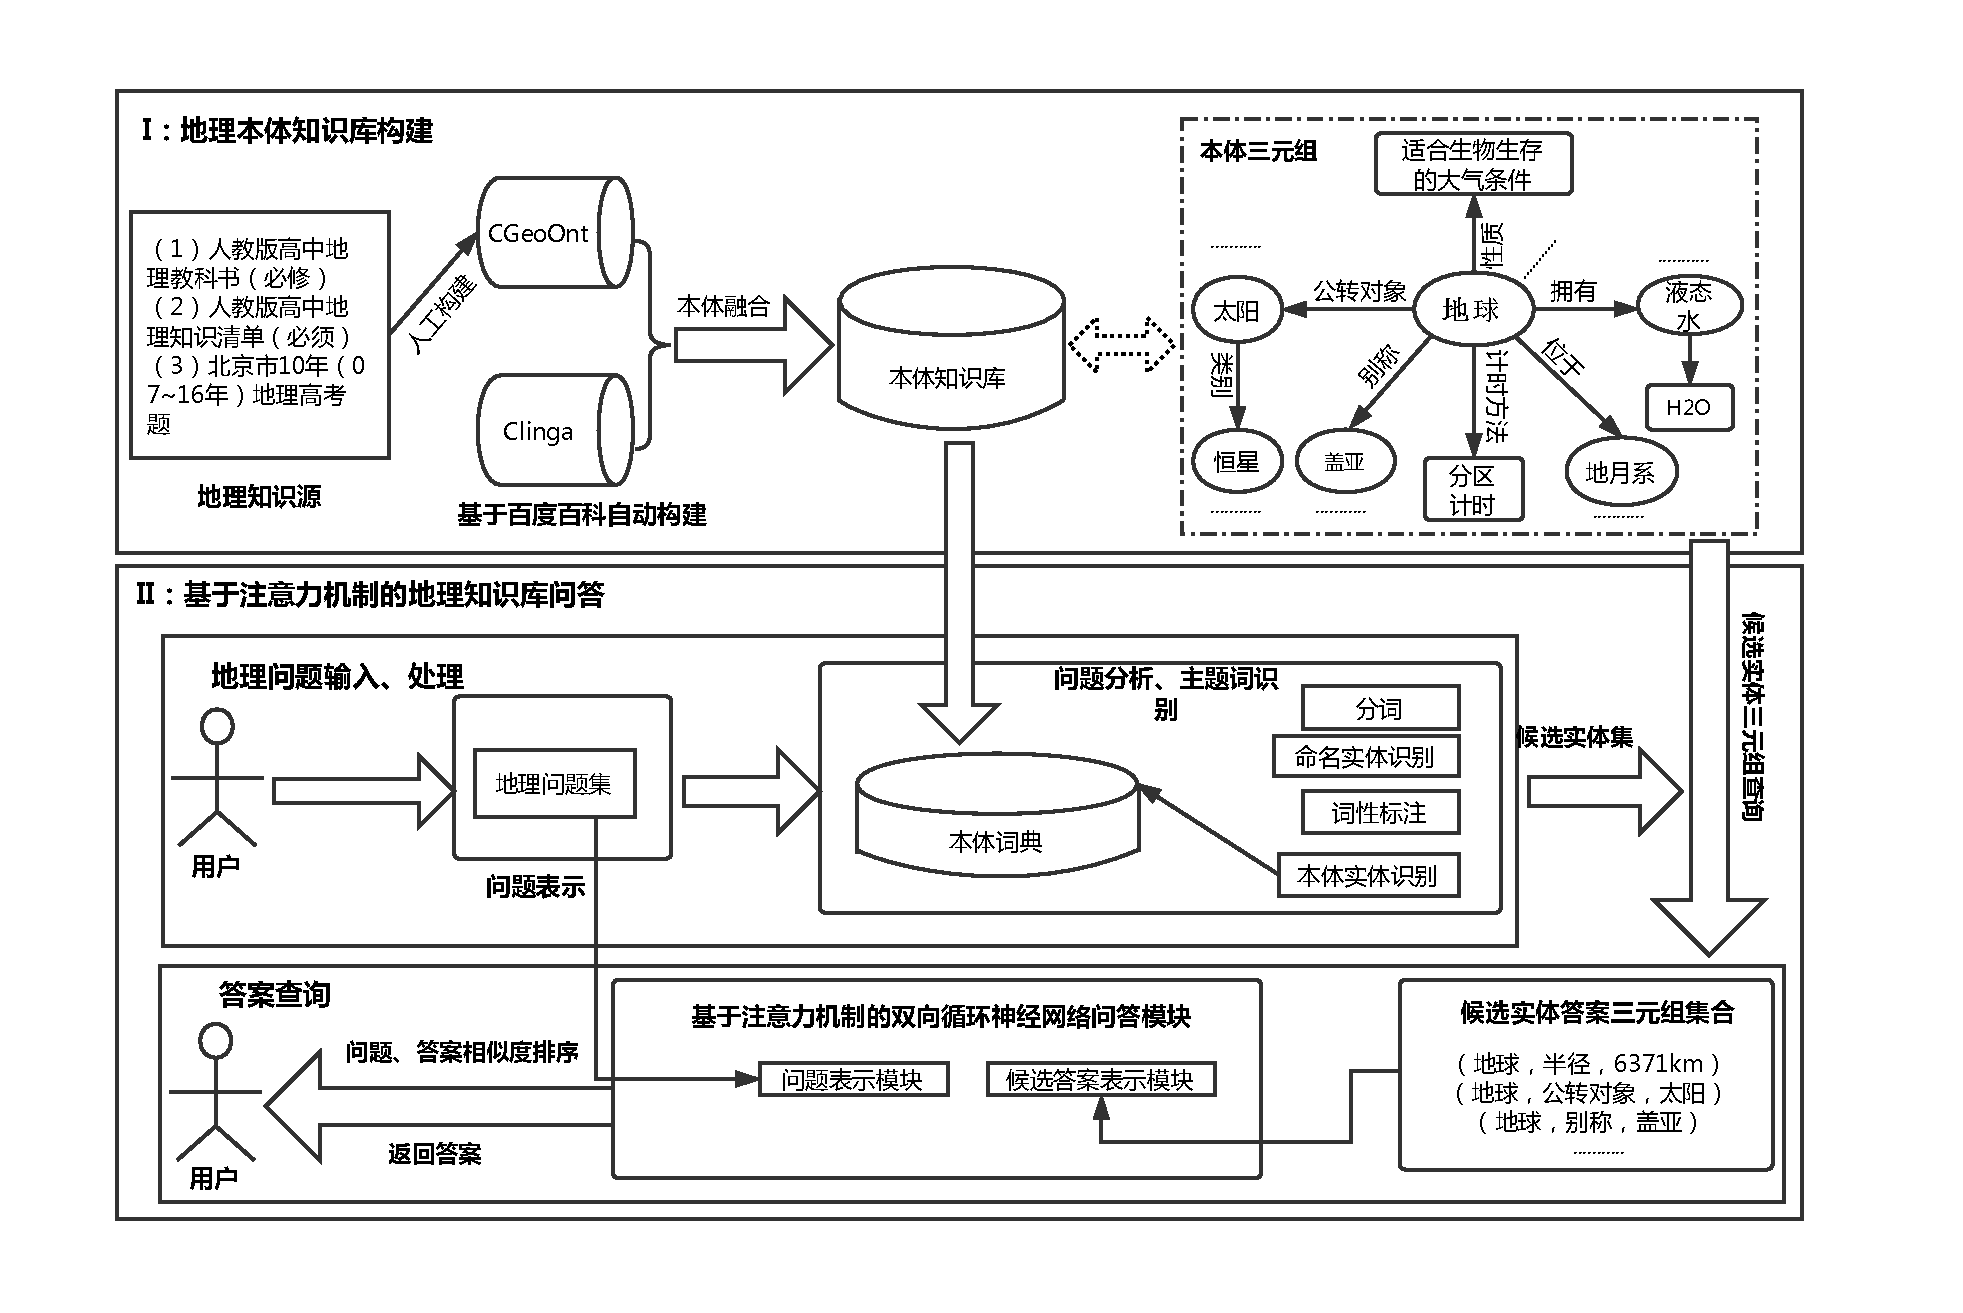
\includegraphics[height=9cm]{resource/graduation}
	\caption{基于本体的地理知识问答系统结构图}
	\label{fig:graduation}
\end{figure}

\section{地理本体知识库构建}
地理本体知识库构建内容分三个部分来介绍,先介绍地理本体CGeoOnt(chinese geographic ontology)的构建,然后介绍本体Clinga(chinese linked geographical dataset)与本体CGeoOnt融合,最后介绍本体词典生成方法。

\subsection{地理本体CGeoOnt构建}\label{section:CGeoOnt_build}
本文本体构建方法借鉴了斯坦福七步法的流程思想,但是与斯坦福的七步法有一些区别,如本文没有可以复用的本体,并且一次性列出本体的重要术语明显可操作性不强。因此,根据本文地理本体构建特点,主要分四个步骤进行构建工作,分别如下:

(1)地理知识源选取。选取本体构建所需要的资料,文档或者图形形式。

(2)地理知识体系定义。确定本体构建的三元组知识组织顺序。

(3)地理本体构建规范定义。约定本体构建的知识组织规范。

(4)地理本体基本元素定义。定义类、属性、关系,创建实例。

\subsubsection{地理知识源选取}
地理本体构建知识源来自专业的高中地理教材以及部分的高考试题。地理教材包括人教版高中地理必修一自然地理、必修二人文地理、必修三区域可持续发展、区域地理、选修三旅游地理、选修五自然灾害与防治、选修六环境保护这七本教材和一本高中地理知识清单。高中地理知识清单是专家对上述七本高中地理教材中核心考点的精确提炼以及每本书知识点的解题方法讲解。高考试题选取的是北京市近10年(2007年~2016年)的地理高考题,选取高考题作为知识源的目的是:标注人员可以根据高考题快速把握高考地理考点以及解决考点所需要的辅助知识,因此可以很有目的性的去教材中寻找需要标注的核心知识,避免标注大量对于解题无用的地理知识,大大提高了地理核心知识库构建的效率。本文地理资源均为电子资源,且格式为HTML的网页形式,里面包含文字叙述、图和表格。

\subsubsection{地理知识体系定义}
地理知识体系的定义根据《高中地理知识清单(第3次修订)》
中的组织结构进行,该高中地理知识清单包括了整个高中地理教科书中知识的组织顺序,如高中地理教材的组织先从必修地理开始,包括必修自然地理、必修人文地理、必须区域可持续发展。然后是介绍选修地理部分,包括选修旅游地理、选修自然灾害与防治和选修环境保护。对于每一本教材中的知识体系根据书中每个章节的相关主题、相关知识点和相关方法三个方面来组织,这样的好处是使知识库的知识都能够找到其知识的出处,便于后续分析知识之间的关系和知识溯源,保留知识的完整性。如在标注概念类“天体”的知识三元组时,需要标注出“天体”在书中所属的“相关主题”是“宇宙中的地球”,以及“天体”涉及的“相关知识点”是“地球的宇宙环境”和跟“天体”相关联的“相关方法”是“天体类型的判断方法”。

\subsubsection{地理本体构建规范}
地理本体构建规范主要为保证最终本体的构建形式一致,因为本体构建需要多个专业人员参与,不同人的标注主观性很大,必须经过统一的规范约束。首先,本文地理知识需要较强的表达能力且还需具备很强的推理能力,因此本文约定本体描述语言使用OWL,构建符合RDFS和OWL DL级别规范。其次,由于本文地理本体构建有很多自己的特殊定义,有些定义需要突破OWL DL的规范,因此本文构建工作不使用当前存在的本体构建工具,如protege等,本文直接以RDF三元组的语法形式Turtle\footnote{https://www.w3.org/TR/turtle/}来表示每条本体知识(三元组)。最后,本文规定个体、类、属性等的命名说明规范,统一本体的最终表现形式。

为简化三元组的表示,本文定义了本文地理本体术语的命名空间,包括自定义的三个地理本体元素——个体、属性及类的命名空间gsr、gss、gso,以及包括七个常见的本体元素命名空间:rdf、rdfs、owl、skos、xs、op和fn。以上命名空间如下所示:

% 用s表示正常的字符宽度,l代表稍微窄的字符宽度

@prefix gsr:\hphantom{sss}<http://ws.nju.edu.cn/geoscholar/resource>.

@prefix gss:\hphantom{sss}<http://ws.nju.edu.cn/geoscholar/staticOntology>.

@prefix gso:\hphantom{ssl}<http://ws.nju.edu.cn/geoscholar/ontology>.

@prefix rdf:\hphantom{sss}<http://www.w3.org/1999/02/22-rdf-syntax-ns>.

@prefix rdfs:\hphantom{ss}<http://www.w3.org/2000/01/rdf-schema>.

@prefix owl:\hphantom{ss}<http://www.w3.org/2002/07/owl>.

@prefix skos:\hphantom{ll}<http://www.w3.org/2004/02/skos/core>.

@prefix xs:\hphantom{sssl}<http://www.w3.org/2001/XMLSchema>.

@prefix op:\hphantom{ssll}<http://www.w3.org/2002/08/xquery-operators>.

@prefix fn:\hphantom{sssl}<http://www.w3.org/2005/xpath-functions>.\linebreak[3]
\\
以下为其他约定,核心思想为本体不同元素有区分度,同时见其英文名可知其中文义:
\begin{itemize}
	\item {个体:以“R\_”开头,如gsr:R\_太阳。
	}
	\item {类:以“C\_”开头,如gso:C\_天体。
	}
	\item{属性(静态属性):以“P\_”开头,两个属性owl:ObjectProperty、owl:DatatypeProperty分别以“P\_o\_”和“P\_d\_”开头。如gso:P\_o\_公转对象,gso:P\_d\_高度。
	}
	\item{个体必须声明类别owl:Class、属性必须确定是对象属性owl:ObjectProperty还是数据类型属性owl:DatatypeProperty。
	}
	\item{每个术语有且仅有一个skos:prefLabel,但是可以有多个skos:altLabel用于别名。
	}
	\item {每个术语有必要时使用skos:definition给出其定义,使用rdfs:comment对其重要方面进行评论。
	}
	\item {术语间多使用gso:relatedTo来表达它们有一定的关联性。
	}
	\item {为避免处理的复杂性,三元组中不使用空白节点( blank node )。
	}
\end{itemize}

\subsubsection{地理本体基本元素定义}
本文地理本体构建遵循自下而上的原则,按照书本知识的组织顺序构建本体,不一次性的定义其领域所有术语,而采取根据每章、每节中的考点知识构建,考点知识的确定参照10年的北京市地理高考题以及书中重点强调的考点。下面分别介绍类、属性、个体和本文特殊地理元素的具体构建。

(1)类的构建

类的构建需要声明其类型是OWL中的类,并且需要定义其唯一的名称skos:prefLabel,而且该类若有别名则需定义别名skos:altLabel,该类的父类(\text{subClassOf})若有则需要定义出。类相关的定义或者评论可以通过skos:definition和skos:comment定义出,并且若该类所对应的课文章节主题和知识点为重要考点,也应该定义出。如下举例为本文对概念类“天体”的三元组知识表示,知识三元组中的主语、谓语、宾语之间以空格表示:

gso:C\_行星\quad rdf:type\quad owl:Class\quad .

gso:C\_行星\quad skos:prefLabel\quad "行星"$^{\land\land}$xs:string\quad .

gso:C\_行星\quad rdfs:subClassOf\quad gso:C\_天体\quad .

gso:C\_行星\quad skos:definition\quad "在椭圆轨道上,环绕恒星运行、近似球状的天体,其质量比恒呈小,本身是不发光的\"$^{\land\land}$xs:string\quad .

gso:C\_行星\quad gsb:relatedToKPoint\quad gsb:M\_太阳对地球的影响\quad .

gso:C\_行星\quad gsb:relatedToKPoint\quad gsb:M\_宇宙中的地球\quad .

gso:C\_行星\quad gsb:relatedToTopic\quad gsb:M\_行星地球 .
\\

(2)属性的构建 

本文的属性包括普通的属性和本文特殊定义的属性,此节只讲述普通属性的构建,特殊定义的属性到第四节“地理特殊定义元素”介绍。本文普通属性的构建前提得明确区分对象属性owl:ObjectProperty和数据类型属性owl:DatatypeProperty,属性的性质(如对称性、传递性等)需要定义出来,便于根据属性进行相关推理。同时,对于对象属性,本文需描述属性的定义域rdfs:domain和值域rdfs:range,不好区分情形下使用总类owl:Thing描述;对于数据类型属性,数据类型的单位必须定义,如下分别为对象属性“垂直”和数据属性“宽度值”的表示:

对象属性:垂直

gso:P\_o\_垂直\quad rdf:type\quad owl:ObjectProperty\quad .(对象属性)

gso:P\_o\_垂直\quad skos:prefLabel\quad "垂直"$^{\land\land}$xs:string\quad .(属性名称)

gso:P\_o\_垂直\quad rdfs:domain\quad owl:Thing\quad .\quad (定义域为所有对象)

gso:P\_o\_垂直\quad rdfs:range\quad owl:Thing\quad .\quad (值域为所有对象)

gso:P\_o\_垂直\quad a\quad owl:SymmetricProperty\quad .\quad \quad (对称性)

gsr:R\_水平气压梯度力\quad gso:P\_o\_垂直\quad gsr:R\_等压线\quad .(属性连接的两个对象)

gso:P\_o\_垂直\quad gsb:relatedToKPoint\quad gsb:M\_大气的水平运动-风\quad .(属性涉及到的考点知识)\\

数据属性:宽度值

gso:P\_d\_宽度值\quad rdf:type\quad owl:DatatypeProperty\quad .(数据属性)

gso:P\_d\_宽度值\quad skos:prefLabel\quad "宽度值"$^{\land\land}$xs:string\quad .(属性名称)

gso:P\_d\_宽度值\quad gso:physicalQuantity\quad "宽度"$^{\land\land}$xs:string\quad .(属性单位名称)

gso:P\_d\_宽度值\quad gso:unit\quad "米"$^{\land\land}$xs:string\quad .(属性单位类型)

gso:P\_d\_宽度值\quad rdfs:domain\quad owl:Thing\quad .(定义域为所有对象)

gso:P\_d\_宽度值\quad rdfs:range\quad xs:double\quad .(值域为双精度数值)

gso:P\_d\_宽度值\quad rdfs:comment\quad "描述某物a的宽度为某个值"$^{\land\land}$xs:string\quad .(属性的一般性评论)

gsr:R\_南极附近海上最大的冰山\quad gso:P\_d\_宽度值\quad \quad "97000.0"$^{\land\land}$xs:double\quad .(属性描述的个体知识)

gso:P\_d\_宽度值\quad gsb:relatedToKPoint\quad gsb:M\_水资源与人类社会\quad .(属性相关的知识考点)

gso:P\_d\_宽度值\quad gsb:relatedToTopic\quad gsb:M\_水资源的合理利用\quad .(属性相关的知识考点章节)  \\

(3)个体的构建

个体的构建只包含标注章节中包含高考地理考点的专业术语,其它非考点术语忽略不予标注。本文个体构建遵循最重要的一个原则就是每个个体必须申明其类别,而且其类别允许为多个,这一点也符合现实世界的表示。如下为术语个体“地球”的知识表示:

gsr:R\_地球\quad skos:prefLabel\quad "地球"$^{\land\land}$xs:string\quad .\quad (个体名称)

gsr:R\_地球\quad rdf:type\quad gso:C\_行星\quad .(个体的类别,此处地球有三个标签类别)

gsr:R\_地球\quad rdf:type\quad gso:C\_物体\quad .(个体的类别)

gsr:R\_地球\quad rdf:type\quad gso:Location\quad .(个体的类别)

gsr:R\_地球\quad gso:P\_d\_性质\quad "适合生物生存的大气条件"$^{\land\land}$xs:string\quad .(个体数据-字符串属性,描述的事实是:地球拥有适合生物生存的大气条件的性质)

gsr:R\_地球\quad gso:P\_d\_轨道偏心率\quad "0"$^{\land\land}$xs:string\quad .(个体数据-字符串属性)

gsr:R\_地球\quad gso:P\_d\_计时方法\quad "分区计时"$^{\land\land}$xs:string\quad .(个体数据-字符串属性)

gsr:R\_地球\quad gso:P\_d\_时区数量\quad "24"$^{\land\land}$xs:integer\quad .(个体数据-整型属性)

gsr:R\_地球\quad gso:P\_d\_平均密度\quad "5"$^{\land\land}$xs:string\quad .(个体数据-字符串属性)

gsr:R\_地球\quad gso:P\_o\_公转对象\quad gsr:R\_太阳\quad .(个体的对象属性)

gsr:R\_地球\quad gso:P\_o\_天然卫星\quad gsr:R\_月球\quad .(个体的对象属性)

gsr:R\_地球\quad gso:P\_o\_拥有\quad gsr:R\_液态水\quad .(个体的对象属性)

gsr:R\_地球\quad gso:P\_o\_南部\quad gsr:R\_南半球\quad .(个体的对象属性)
\\

(4)地理本体特色元素

$\P$静态属性
		
静态属性,本文前缀表示为gss,是为增强地理知识的表达能力而设定的,需与普通属性gso相区别。静态属性严格上并不满足OWL的属性规范,因为OWL的属性连接的可以是两个个体或者一个个体一个数据类型数据,而本文的静态属性描述的是类的属性特征。静态属性重要的特性是静态属性所描述的类所包含的所有个体均具有该静态属性特征,这一点类似于个体继承类的特征。由于静态属性是对一类个体的描述,本文可以允许其不申明定义域rdfs:domain和值域rdfs:range,但是该静态属性仍然区分是对象属性owl:ObjectProperty还是数据类型属性owl:DatatypeProperty,如下对类“暖流”定义了一个静态属性“作用”。

gss:P\_d\_作用\quad rdf:type \quad owl:DatatypeProperty\quad .(gss申明静态数据类型属性)

gso:C\_暖流\quad gss:P\_d\_作用\quad "对沿岸气候增温增湿"$^{\land\land}$xs:string\quad .

gsr:R\_北大西洋暖流\quad rdf:type\quad gso:C\_暖流.(申明暖流的个体-北大西洋暖流)
\\
则表明:北大西洋暖流同样具有暖流的静态属性特性,也即:

gsr:R\_北大西洋暖流\quad gso:P\_d\_作用\quad "对沿岸气候增温增湿"$^{\land\land}$xs:string\quad .
	\\
	
$\P$封闭集

封闭集用符号gso:isClosed表示,包括类和属性的封闭集。类的封闭集表示某个类的实例可以全部列举出,属性的封闭集表示某个个体在该属性上取值是封闭的,即包含有限的取值且可以穷举出来。

	$\bullet$类封闭集知识举例:地球的极点包括南极点、北极点

gsr:R\_北极点\quad a\quad gso:C\_地球极点\quad .

gsr:R\_南极点\quad a\quad gso:C\_地球极点\quad .

gso:C\_地球极点\quad gso:isClosed\quad "true"$^{\land\land}$xs:boolean\quad .

地球极点类在封闭集gso:isClosed属性上取值为true,说明地球极点的取值实例个体已经完整了,只有南极点和北极点。

$\bullet$属性封闭集知识举例:太阳大气层由里到外可分为光球、色球、日冕三层。

gsr:R\_太阳大气层\quad gso:P\_o\_包含\quad gsr:R\_光球\quad ;

gsr:R\_太阳大气层\quad gso:P\_o\_包含\quad gsr:R\_色球\quad ;

gsr:R\_太阳大气层\quad gso:P\_o\_包含\quad gsr:R\_日冕\quad .

gso:P\_o\_包含\quad gso:isClosedAt\quad gsr:R\_太阳大气层\quad.

该知识表示“包含”属性在个体“太阳大气层”上处于封闭状态,说明太阳大气层只包括光球、色球和日冕三层。
	\\

$\P$地理数值类型

常见的数值类型属性的取值都较为明确,如使用整型xs:integer,双精度浮点型xs:double来表示。然而,在地理学科中,大多数出现的数值都不是精确值,往往是某种程度上的近似值。下面介绍本文几种类型的近似值处理介绍:

$\bullet$约取值

约取值的主要描述特征为“某某约为多少”,此种情况本文视作精确值处理,如知识:太阳表面的温度大约为6000K,直接取6000K作为温度数值,表示如下:

gsr:R\_太阳\quad gso:P\_d\_表面温度\quad "6000"$^{\land\land}$xs:decimal .
\\

$\bullet$表示“几”

对于地理知识源中包含“几”的数值描述,本文使用两种方法进行标注,第一种是查阅相关的权威资料,了解其具体的值;第二种是在无法通过其它辅助资料查询到相关精确数值时,使用1~9加上单位的范围值表示。如下两种举例:

地理知识:色球厚度约为几千千米,实际上通过查阅维基百科可以发现,“色球厚度大约是2,000公里”,因此可以表示如下:

gsr:R\_色球\quad gso:P\_d\_厚度\quad “2e6”$^{\land\land}$xs:double\quad .

如果无法查阅其他资料得到准确值,则采取范围区间值来表示,如下:

gsr:R\_色球\quad gso:P\_d\_厚度\quad "(1e6, 9e6)"$^{\land\land}$\quad xs:impreciseInterval\quad .
\\

$\bullet$范围值

本文标注过程中主要遇到三种范围值的表述,第一种为取值唯一,但不精确,第二种为条件缺省时导致的取值不确定,第三种为无法精确到确定的取值区间。

第一种范围值使用不精确的区间值xs:impreciseInterval表示,以圆周率举例,圆周率的值为3.1415926~3.1415927范围之间。或者再如地理知识:崇明岛全岛的面积为1200多平方千米,可以表示如下:

gsr:R\_崇明岛\quad gso:P\_d\_面积值\quad "(1.201e9, 1.299e9)"$^{\land\land}$xs:impreciseInterval\quad .

第二种范围值使用不明确的区间值xs:unclearInterval表示,如日地距离的取值,(时间不同时,日地距离亦不同),某省某刻的温度(具体的地点不同时,温度也不同)。这样的例子当补充了具体的条件,如具体时间、具体地点后就有可能转换为精确值。本文把此种复杂的条件限制使用最低到最高的区间值来表示,如下表示地球大气上界的高度不同时间的范围值:

gsr:R\_地球大气上界\quad gso:P\_d\_高度\quad "(2e6,  3e6)"$^{\land\land}$xs:unclearInterval\quad .

第三种使用不能被精确为确定值的区间xs:scopeInterval表示,如没有最大值的开区间,以地理知识为例:亚热带季风气候年降水量在800mm以上,范围值只有下界值,没有上界值,因此此种形式本文使用开区间表示,如下:


gsr:R\_亚热带季风气候\quad gso:P\_d\_年降水量\quad "[0.8, )"$^{\land\land}$xs:scopeInterval\quad .
\\

$\bullet$地理区域表示

地理区域主要指存在于空间中且可以准确定位的空间位置。地理中常常考察地理地点之间的位置关系(接壤、方向、包含等),因此对于地理重要地点的位置表示,需要准确细致的刻画。本文将空间所有事物定义为一个大类,记作gso:SpatialThing,将可以空间定位的地点定义为空间事物类的子类,记作gso:Location。如下先介绍空间位置关系,后介绍利用空间关系来表示空间位置。

空间关系:

空间关系用于描述两个可定位地点位置的相对方位关系,从某种程度上来看它也是一种对象属性,表达两个空间位置的关系。本文定义的位置关系都符合地理领域的方位表达方式,本文以常见的方位关系“位于”、“中部”来说明。“位于”表示一个位置在另一个位置上,属于一直包含的关系。“中部”表示对一个位置的方向约束,如中国中部等。如下为具体的地理知识表示:“基拉韦厄火山位于北太平洋中部的夏威夷群岛上”,本文需要准确表示出“位于”关系,北太平洋中部和被太平洋的方位“中部”关系

gsr:R\_基拉韦厄火山\quad rdf:type\quad  gso:Location\quad  .

gsr:R\_夏威夷群岛\quad rdf:type\quad  gso:Location\quad  .

gsr:R\_北太平洋\quad rdf:type\quad  gso:Location\quad  .

gsr:R\_北太平洋中部\quad rdf:type\quad  gso:SpatialThing\quad  .

gsr:R\_基拉韦厄火山\quad  gso:P\_o\_位于\quad  gsr:R\_夏威夷群岛\quad  .

gsr:R\_夏威夷群岛\quad  gso:P\_o\_位于\quad  gsr:R\_北太平洋中部\quad  .

gsr:R\_北太平洋\quad  gso:P\_o\_中部\quad  gsr:R\_北太平洋中部\quad  .
\\

空间位置:

对于空间位置,尤其是需要通过复杂空间关系来表示的空间位置,先得将其声明为gso:SpatialThing的实例,然后通过空间关系属性(谓词),建立与其他空间位置的关系,最后通过与其它位置构成的关系来整体表示该空间位置。如地理知识:“亚热带季风气候分布地区为我国秦岭-淮河以南、朝鲜半岛南部、日本群岛南部”,该知识中包含的“秦岭-淮河以南”、“朝鲜半岛南部”和“日本群岛南部”这三个带有方向限定的位置,需以本文定义的空间关系“南方”、“南部”并结合具体位置来联合表示,比如“秦岭-淮河以南”需要定义为“秦岭-淮河”的空间关系“南方”,具体表示如下:

gsr:R\_秦岭-淮河\quad rdf:type\quad gso:Location\quad .

gsr:R\_日本群岛\quad rdf:type\quad gso:Location\quad .

gsr:R\_朝鲜半岛\quad rdf:type\quad gso:Location\quad .

gsr:R\_秦岭-淮河以南\quad rdf:type\quad gso:SpatialThing\quad .

gsr:R\_日本群岛南部\quad rdf:type\quad gso:SpatialThing\quad .

gsr:R\_朝鲜半岛南部\quad rdf:type\quad gso:SpatialThing\quad .

gsr:R\_秦岭-淮河\quad gso:P\_o\_南方\quad gsr:R\_秦岭-淮河以南\quad .

gsr:R\_日本群岛\quad gso:P\_o\_南部\quad gsr:R\_日本群岛南部\quad .

gsr:R\_朝鲜半岛\quad gso:P\_o\_南部\quad gsr:R\_朝鲜半岛南部\quad .

gsr:R\_亚热带季风气候\quad gso:P\_o\_分布地区\quad gsr:R\_秦岭-淮河以南\quad ,\quad 

gsr:R\_亚热带季风气候\quad gso:P\_o\_分布地区\quad gsr:R\_日本群岛南部\quad ,\quad 

gsr:R\_亚热带季风气候\quad gso:P\_o\_分布地区\quad gsr:R\_朝鲜半岛南部\quad .
\\
再如“接壤”位置之间的表示,如知识:“亚欧板块和太平洋板块的交界处地震多发
”,需要表现“亚欧板块”与“太平洋板块”的"相接"也即“接壤”关系。

gsr:R\_亚欧板块\quad rdf:type \quad gso:Location\quad .

gsr:R\_太平洋板块\quad rdf:type \quad gso:Location\quad .

gsr:R\_亚欧板块\quad gso:P\_o\_相接\quad gsr:R\_太平洋板块\quad .

gsr:R\_亚欧板块和太平洋板块的交界处\quad rdf:type \quad gso:SpatialThing\quad ;\quad 

gsr:R\_亚欧板块和太平洋板块交界处\quad gso:P\_o\_相接\quad gsr:R\_亚欧板块\quad ;

gsr:R\_亚欧板块和太平洋板块交界处\quad gso:P\_o\_相接\quad gsr:R\_太平洋板块\quad ;

gsr:R\_亚欧板块和太平洋板块交界处\quad gso:P\_d\_地震发生率\quad "多"^^xs:string .
\\

$\bullet$过程表示

本文过程是指地理中一些现象在一系列条件下通过一系列步骤而形成的总称,常常有顺序过程和循环过程。本文将过程定义为一个大类gso:Process,然后顺序过程gso:SequentialProcess和循环过程CircularProcess分别申明为其子类。对于顺序过程或者循环过程,都需要严格的定义其形成所需要的步骤,以及每个步骤上面的步骤条件。具体定义如下:\\
先申明类:

gso:Process\quad rdf:type\quad owl:Class\quad .\quad (过程类)

gso:CircularProcess\quad rdfs:subClassOf\quad gso:Process\quad .(循环型过程类)

gso:SequentialProcess\quad rdfs:subClassOf\quad gso:Process\quad .\quad (顺序型过程类)

gso:StepOfProcess\quad rdf:type\quad owl:Class\quad .(过程的步骤类)
\\
再申明条件、步骤属性:

gso:condition4Step\quad rdf:type\quad owl:DatatypeProperty\quad .\quad (步骤条件,值为字符串)

gso:condition4Step\quad rdfs:domain\quad gso:StepOfProcess\quad .

gso:stepDesc\quad rdf:type\quad owl:DatatypeProperty\quad .\quad (步骤文字描述,取值为字符串)

gso:stepDesc\quad rdfs:domain\quad gso:StepOfProcess\quad .

gso:stepNum\quad rdf:type\quad owl:DatatypeProperty\quad .\quad (步骤的序号,第几个步骤,取值为正整数)

gso:stepNum\quad rdfs:domain\quad gso:StepOfProcess .

如下复杂地理过程知识的具体表示:“冷锋过境前,会受单一暖气团的控制,温暖晴朗。当冷气团主动移动向暖气团时,较重的冷气团会插入暖气团下面,使暖气团被迫的抬升。暖气团在抬升的过程中逐渐的冷却,其中水汽易凝结成云。如果暖空气中含有大量水汽,那么可能会导致雨雪天气。冷锋移动速度较快,常常带来较强的风。冷锋过境后,冷气团替代原来暖气团的位置,气压升高,气温降低,湿度骤降,天气则转好。”

上述叙述的是地理现象“冷锋过境”的形成过程,如下具体表示:\\
先申明“过程”和“步骤”:

gsr:R\_冷锋过境过程\quad rdf:type\quad \quad gso:SequentialProcess\quad .

gsr:R\_冷锋过境过程\quad gso:numberOfSteps\quad "3"$^{\land\land}$xs:positiveInteger\quad .

gsr:R\_冷锋过境步骤\_1\quad rdf:type\quad \quad gso:StepOfProcess\quad .

gsr:R\_冷锋过境步骤\_2\quad rdf:type\quad \quad gso:StepOfProcess\quad .

gsr:R\_冷锋过境步骤\_3\quad rdf:type\quad \quad gso:StepOfProcess\quad .

gsr:R\_冷锋过境过程\quad gso:includesStep\quad gsr:R\_冷锋过境步骤\_1\quad ,\quad 

gsr:R\_冷锋过境过程\quad gso:includesStep\quad gsr:R\_冷锋过境步骤\_2\quad ,\quad 

gsr:R\_冷锋过境过程\quad gso:includesStep\quad gsr:R\_冷锋过境步骤\_3\quad .
\\
再申明“步骤”的文字描述gso:stepDesc和条件gso:condition4Step:

gsr:R\_冷锋过境步骤\_1\quad gso:stepNum\quad "1"$^{\land\land}$xs:positiveInteger\quad ;

gso:stepDesc\quad "当冷气团主动移向暖气团时,较重的冷气团插入暖气团下面,使暖气团被迫抬升。"$^{\land\land}$xs:string\quad .

gsr:R\_冷锋过境步骤\_2\quad gso:stepNum\quad "2"$^{\land\land}$xs:positiveInteger\quad ;

gsr:R\_冷锋过境步骤\_2\quad gso:stepDesc\quad "暖气团在抬升过程中逐渐冷却,其中水汽容易凝结成云。"$^{\land\land}$xs:string\quad .

gsr:R\_冷锋过境步骤\_3\quad gso:stepNum\quad "3"$^{\land\land}$xs:positiveInteger\quad ;

gsr:R\_冷锋过境步骤\_3\quad gso:condition4Step\quad "暖空气中含有大量水汽。"$^{\land\land}$xs:string\quad ;

gsr:R\_冷锋过境步骤\_3\quad gso:stepDesc\quad "如果暖空气中含有大量的水汽,那么可能会带来雨雪天气。"$^{\land\land}$xs:string\quad .

此“冷锋过境”过程中实际上也包含了不同时段的“天气变化”,因此“冷锋过境中的天气变化”也需要表示为一个顺序过程,这样在考察“冷锋过境”与天气变化的关系是,可以运用此结构化的知识表示。具体表示如下:
\\
申明“冷锋过境中的天气变化”为顺序过程:

gsr:R\_冷锋过境中的天气变化\quad rdf:type \quad gso:SequentialProcess\quad ;

gsr:R\_冷锋过境中的天气变化\quad gso:numberOfSteps\quad "3"$^{\land\land}$xs:positiveInteger\quad .

gsr:R\_冷锋过境中天气变化的步骤\_1\quad rdf:type \quad gso:StepOfProcess\quad .

gsr:R\_冷锋过境中天气变化的步骤\_2\quad rdf:type \quad gso:StepOfProcess\quad .

gsr:R\_冷锋过境中天气变化的步骤\_3\quad rdf:type \quad gso:StepOfProcess\quad .

gsr:R\_冷锋过境过程中的天气变化\quad gso:includesStep\quad gsr:R\_冷锋过境中天气变化的步骤\_1\quad ,\quad 

gsr:R\_冷锋过境过程中的天气变化\quad gso:includesStep\quad gsr:R\_冷锋过境中天气变化的步骤\_2\quad ,\quad 

gsr:R\_冷锋过境过程中的天气变化\quad gso:includesStep\quad gsr:R\_冷锋过境中天气变化的步骤\_3\quad .
\\
申明“冷锋过境中的天气变化”的每个步骤的内容和条件:

gsr:R\_冷锋过境中天气变化的步骤\_1\quad gso:stepNum\quad "1"$^{\land\land}$xs:positiveInteger\quad ;

gsr:R\_冷锋过境中天气变化的步骤\_1\quad gso:condition4Step\quad "过境前"$^{\land\land}$xs:string\quad ;

gsr:R\_冷锋过境中天气变化的步骤\_1\quad gso:stepDesc\quad "过境前,单一暖气团控制,温暖晴朗。"$^{\land\land}$xs:string\quad .

gsr:R\_冷锋过境中天气变化的步骤\_2\quad gso:stepNum\quad "2"$^{\land\land}$xs:positiveInteger\quad ;

gsr:R\_冷锋过境中天气变化的步骤\_2\quad gso:condition4Step\quad "过境时"$^{\land\land}$xs:string\quad ;

gsr:R\_冷锋过境中天气变化的步骤\_2\quad gso:stepDesc\quad "过境时,常有阴天、下雨、刮风、降温等天气现象。"$^{\land\land}$xs:string\quad .

gsr:R\_冷锋过境中天气变化的步骤\_3\quad gso:stepNum\quad "3"$^{\land\land}$xs:positiveInteger\quad ;

gsr:R\_冷锋过境中天气变化的步骤\_3\quad gso:condition4Step\quad "过境后"$^{\land\land}$xs:string\quad ;

gsr:R\_冷锋过境中天气变化的步骤\_3\quad gso:stepDesc\quad "过境后,气强和湿度骤降,天气转睛。"$^{\land\land}$xs:string\quad .

\subsection{地理本体融合}
本文地理核心知识库由构建的两个本体融合而成。这两个本体分别是本文手工构建的CGeoOnt和863项目组基于百度百科自动构建的本体Clinga。本节先介绍Clinga的相关情况,后介绍两个地理本体的融合方法。

\subsubsection{本体Clinga}

本体Clinga\footnote{http://ws.nju.edu.cn/clinga/}为863项目组Hu【26】等人根据百度百科自动抽取构建的中文地理链接数据集(Chinese linked geographical dataset)。Clinga的本体Schema为Hu等人人工根据地理领域特点来定义,他们将地理分为自然地理和人文地理两个大类,然后在这两个大类下再依次细分为多个小类,最后形成Clinga的schema,具体如摘要图\ref{fig:clinga}所示。通过定义好的本体schema对自动抽取到的百度百科概念做分类,只选取满足定义好的本体schema类别的实体,最后对每个百科概念页面结构化成三元组形式,最终得到包含624,391个实体概念、130个类别、73,326,425个三元组的本体。Clinga中知识的组织形式为主、谓、宾,即( s, p, o)三元组。例如( A6906464, 公转对象,A6768329)表示“地球绕着太阳公转”, A6906464和 A6768329 分别对应地球、太阳在知识库中的存储ID,“公转对象”表示地球和太阳的一种属性关系。

\begin{figure}[!htb]
	\centering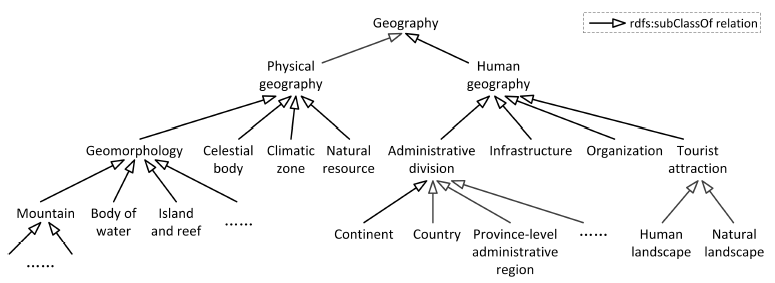
\includegraphics[height=5cm]{resource/clinga}
	\caption{Clinga本体层次结构定义摘要}
	\label{fig:clinga}
\end{figure}

图\ref{fig:clinga}仅仅为Clinga本体结构的一个摘要,有向图的跟节点为总大类地理,然后箭头被指向的是其两个子类自然地理和人文地理,然后依次为这两个子类的定义,依次类推,实际图中的类共有130个,其中的35个叶子类为GeoNames\footnote{http://www.geonames.org/}中没有的类,更具体的情况请参加Hu等人的工作。

\subsubsection{地理本体融合方法}
Clinga 与 CGeoOnt 的 Schema 定义存在一定差异,本文需要将这两个本体进行融合得到一个更综合的地理知识库。本文构建的CGeoOnt 包含类和属性3,000 余个,相关 RDF 三元组 25,000 余条,概念类的定义粒度相比Clinga来说比较细。由于CGeoOnt 本体相对量较小,本文采取将本体CGeoOnt的Schema映射到Clinga的Schema上,具体操作流程如下:

( 1) Clinga 中实体只保留其在百度百科 infobox 域中信息三元组,去掉其 section 文本三元组。

( 2) 运用启发式规则,根据 CGeoOnt 中实体的名称将其类别映射到 Clinga 中的类别。如, CGeoOnt中“黄山”会被映射到 Clinga 中的类 “山”。

( 3) 人工校验( 2) 中映射结果。

( 4)得到最终本体知识库三元组 4,850,435 条。

\subsection{地理本体词典生成}
本文需要根据构建的地理知识库生成地理概念词典,这些概念包含知识库中的实体和类及两者的同义词。生成的地理本体词典主要用于判断某个命名实体是否属于本文地理知识库的范畴,以便提供相关候选实体的知识库信息,同时也为了查询同一个实体的不同别名。

地理本体词典的生成主要工作为抽取地理概念的同义词,由于本文的知识库有两部分数据来源,分别是本体Clinga和本体CGeoOnt。Clinga中的概念抽取自百度百科,因此可以通过规则模板来抽取某个概念的同义词,本文统计发现属性名为中文名、英文名、外文名、原名、别名、中文名称、其他名称、别称和又叫的均可以当作概念的同义词。由于百科知识组织的主观性强,有的实体在表示时后面常常跟有括号,如“地球 别名 盖亚(Gaia)”,针对此种情况需要将别名值中带有括号的部分也抽取出来,并作为该概念的同义词,如此处的Gaia也作为地球的同义词。CGeoOnt中的同义词已经被标注人员标注出,只需要抽取概念的skos:altLabel属性就可以找出该概念的同义词。通过上述,方法,本文得到共包含75,1103个概念同义词词典。

\section{基于注意力机制的地理知识库问答}
基于注意力机制的中文地理知识库问答指根据本文构建的中文地理知识库,运用基于注意力机制的双向循环神经网络问答模型,对用户提出的地理问题,从知识库搜索出问题答案三元组的总过程。该系统问答流程如图\ref{fig:qa_overview},图\ref{fig:qa_overview}表示的是地理问题“2016年北京处暑节气是什么时间”被回答的流程。首先任务是识别该地理问题中的主题实体,也就是问题是围绕哪个实体概念在提问的,如此问题中考察的是“北京的处暑节气时间”,是考察跟“北京”相关的事实性知识,因此“北京”为主题实体。然后,根据主题实体“北京”从本文构建的知识库中查询出与“北京”直接相连的所有实体作为候选实体,此处为首尔和华盛顿。最后使用双向循环神经网络对此问题和候选答案三元组-北京、首尔、华盛顿的三元组进行词向量表示,取问题与候选答案三元组相似度最大的作为该问题的答案。

总结本文知识库问答任务分为如下四步进行:

\begin{figure}[!htb]
	\centering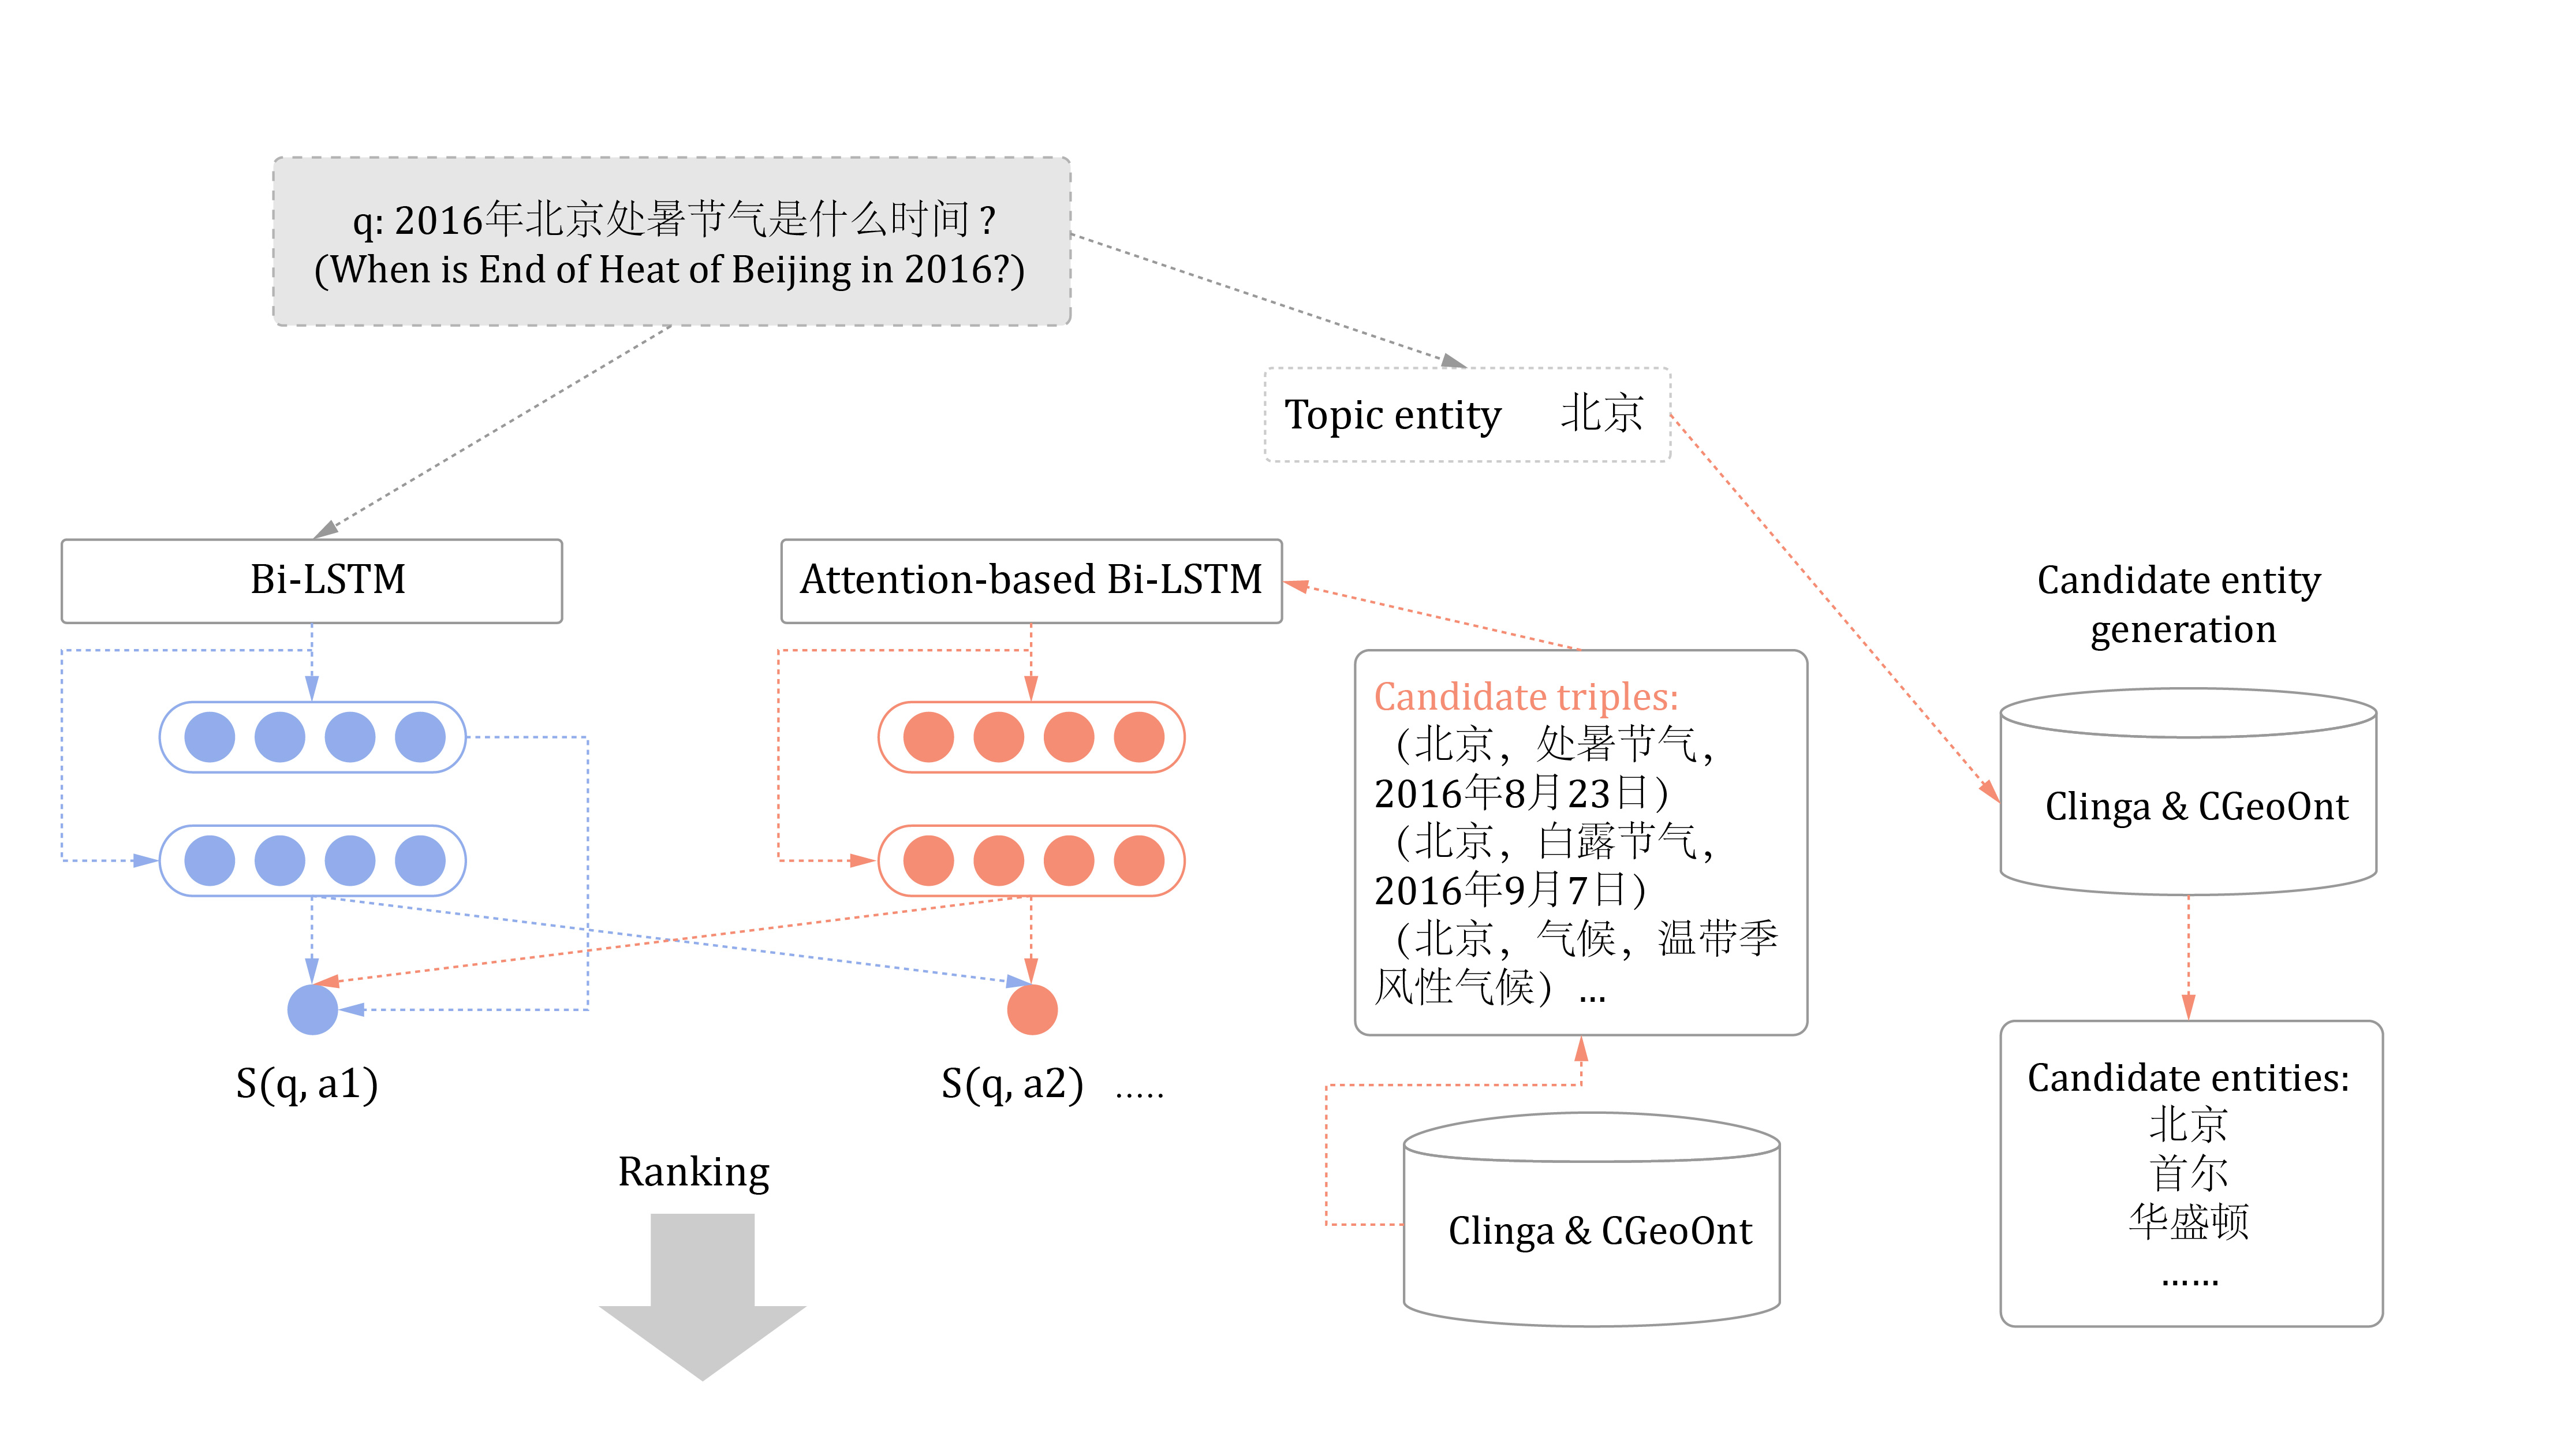
\includegraphics[height=7cm]{resource/qa_overview}
	\caption{基于注意力机制的地理知识库问答流程}
	\label{fig:qa_overview}
\end{figure}

( 1)识别地理问题中涉及的主题实体,根据主题实体生成候选实体集。

(2)根据候选实体集查询知识库,返回候选实体三元组。

( 3)使用双向 LSTM 神经网络编码问题(问题词序列表示成词向量),使用基于注意力机制的双向 LSTM编码候选答案三元组。

( 4)计算问题与每个候选答案三元组的余弦相似度值,返回余弦值最大的三元组作为最终答案(有时返回多个最终答案, 详见 3.4)。

\subsection{地理知识库问答实现方法}
此部分首先介绍候选答案实体三元组的生成方法,然后介绍本文表示问题、答案的基本模型 LSTM,再到其变种双向 LSTM 和结合注意力机制的双向LSTM 模型,最后介绍模型的训练方法和问答最终答案的选择策略。

\subsubsection{候选答案实体三元组生成}
生成候选实体三元组需要识别问题中的主题实体,主题实体也应当存在于本文所使用的知识库中,如果知识库中不存在此主题实体,则问题回答失败。

本文根据知识库构建实体概念词典以及实体概念别名词典,确定知识库能够回答的实体问题范围。候选答案实体三元组生成的关键是识别出问题中的主题实体,如下(1)-—)主题实体识别流程,(4)-(5)步为根据主题实体生成候选答案实体三元组:

(1)使用分词工具jieba\footnote{https://pypi.org/project/jieba/}将问题进行分词,生成句子的词序列。

(2)对词序列进行命名实体识别(Named Entity Recognition, NER)、词性标注(Part  of  Speech, POS), 识别其中的命名实体、名词以及名词词组,本文成为候选主题实体集。

(3)遍历(2)步中生成的候选主题实体集,查询该候选实体是否在本文本体词典中,若存在,则该实体视作主题实体;若为本体词典中词的字串(不包含相等的情况),亦将该实体视作主题实体;若所有候选主题实体都不存在于本体词典中,则本问题没有主题实体,此题目超出本文知识库的回答范围。

(4)从本文地理知识库中获取跟主题实体一跳1-hop\footnote{1-hop表示跟实体距离为1的实体,距离即相连的关系边}和二跳2-hop的实体集合作为候选答案实体集。

(5)最后,从知识库查询出候选答案实体集每个实体的三元组信息,构成目标候选答案实体三元组集合。


\subsubsection{3.1.2\quad 地理问题、候选答案表示}
本节讲述如何将地理问题和候选答案这样的文本序列表示成词向量(word embedding)形式。本文表示地理和候选答案的基础模型为循环神经网络( Recurrent Neural Networks,RNN),本节介绍使用RNN的变种LSTM模型来表示地理问题和答案,本文先介绍RNN表示序列数据的原理,后依次介绍使用基于基本的LSTM表示问题、答案,基于Bi-LSTM来表示问题答案和基于Attention的Bi-LSTM表示答案。
\\

$\P$ RNN表示序列数据原理

RNN的网络结构如图\ref{fig:rnn_structure}所示,图的左边部分表示RNN的循环结构图,RNN的主体结构单元A处理来自当前时刻的输入$x_{i}$和上一时刻A输出的隐含状态。图的右边是左边图的展开形式。RNN中每一层不仅输出$h_{i}$到下一层,而且同时还输出一个隐含状态(hidden state),该隐含状态表示到当前层到前面所有层的保存信息,可以形象化地理解为当前到之前层的所有信息的综合记忆,下一层可以利用上一层输出的隐含状态信息。因此,RNN的这种网络特征结构也使得其非常时候处理前后有依赖关系的数据序列。

\begin{figure}[!htb]
	\centering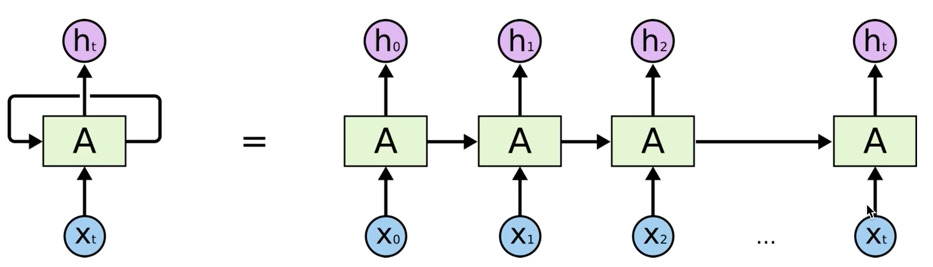
\includegraphics[height=3cm]{resource/rnn_structure}
	\caption{RNN网络结构}
	\label{fig:rnn_structure}
\end{figure}

$\P$基于基本LSTM的表示

在实际中,对于文本序列来说,循环神经网络较难捕捉两个时刻距离较大的文本元素(字或词)之间的依赖关系。LSTM 是 RNN 的变种之一,是一种常用的门控循环神经网络,可以解决 RNN 中的梯度消失、梯度爆炸问题。本文实现的 LSTM 为基于Graves[23]等人改进的 LSTM。给定输入问句,令其序列 \textbf{x}={x(1),x(2),…x(n)}其中 x(t)为问句中每个词的 d 维词向量表示,隐藏单元向量\textbf{$h_{t}$}遵循如下更新方式:

$$
i_t = \sigma(\textbf{W}_{ix}\textbf{x}(t) + \textbf{W}_{ih}\textbf{h}(t - 1) + \textbf{b}_i)
\eqno(1)
$$
$$
f_t = \sigma(\textbf{W}_{fx}\textbf{x}(t) + \textbf{W}_{fh}\textbf{h}(t - 1) + \textbf{b}_f)
\eqno(2)
$$
$$
o_t = \sigma(\textbf{W}_{ox}\textbf{x}(t) + \textbf{W}_{oh}\textbf{h}(t - 1) + \textbf{b}_o)
\eqno(3)
$$
$$
\tilde{C}_t = \tanh(\textbf{W}_{cx}\textbf{x}(t) + \textbf{W}_{ch}\textbf{h}(t - 1) + \textbf{b}_c)
\eqno(4)
$$
$$
C_t = i_t \odot \tilde{C}_t + f_t \odot C_{t-1}
\eqno(5)
$$
$$
\textbf{h}_t = o_t \odot \tanh (C_t)
\eqno(6)
$$

此 LSTM结构通过三个门,输入门 i、输出门 o、遗忘门 f 和记忆单元 c 来控制该时刻前的历史信息是否被记忆、是否需要更新,从而更好的对历史信息进行保存,供下一时刻使用。公式中的$\textbf{W}_{ix}$、 $\textbf{W}_{ih}$、$\textbf{W}_{fx}$、$\textbf{W}_{fh}$、$\textbf{W}_{ox}$、$\textbf{W}_{oh}$、$\textbf{W}_{cx}$、$\textbf{W}_{ch}$、$\textbf{W}_{cx}$、$\textbf{W}_{ch}$、是可学习的权重参数,$\textbf{b}_i$、$\textbf{b}_f$、$\textbf{b}_o$、$\textbf{b}_c$是可学习的偏移参数,$\textbf{h}(t - 1)$为上一时刻的隐含状态输出值,函数σ为sigmoid激活函数,tanh为双曲正切函数作为激活函数,$\tilde{C}_t$表示长短期记忆中的候选记忆单元值,$C_t$为当前时刻的记忆单元值,$C_{t-1}$为当前时刻的记忆单元值,$\odot$为按元素乘法符。

本文首先通过分词将问题转化为词序列,此处记作 $\textbf{q}$ = (x(1), x(2),…x(n)), x(i)表示问题词序列第 i个词, 然后查询词向量矩阵(初始为根据中文维基百科训练得到)获得每个词的初始词向量,最后将序列的词向量输入到上述 LSTM 模型,遵循其更新法进行训练,得到序列最终的词向量。
\\

$\P$基于Bi-LSTM的问题、答案表示

单向 LSTM 模型只考虑当前输入之前的信息,没有考虑其之后输入的信息,往往一个词的含义需要综合考虑此词的前后两部分词信息。因此,本文使用 Bi-LSTM,综合考虑当前输入的前向和后向输出信息, 隐藏单元为前向$\overrightarrow{h_t}$、后向单元$ \overleftarrow{h_t}$相连接,如公式 7 所示:
$$
h_t = (\overrightarrow{h_t}, \overleftarrow{h_t})
\eqno(7)
$$
因此,本文基于 LSTM 的问答模型可以表示为图\ref{fig:qa_bi_lstm}问答模型所示。 
\begin{figure}[!htb]
	\centering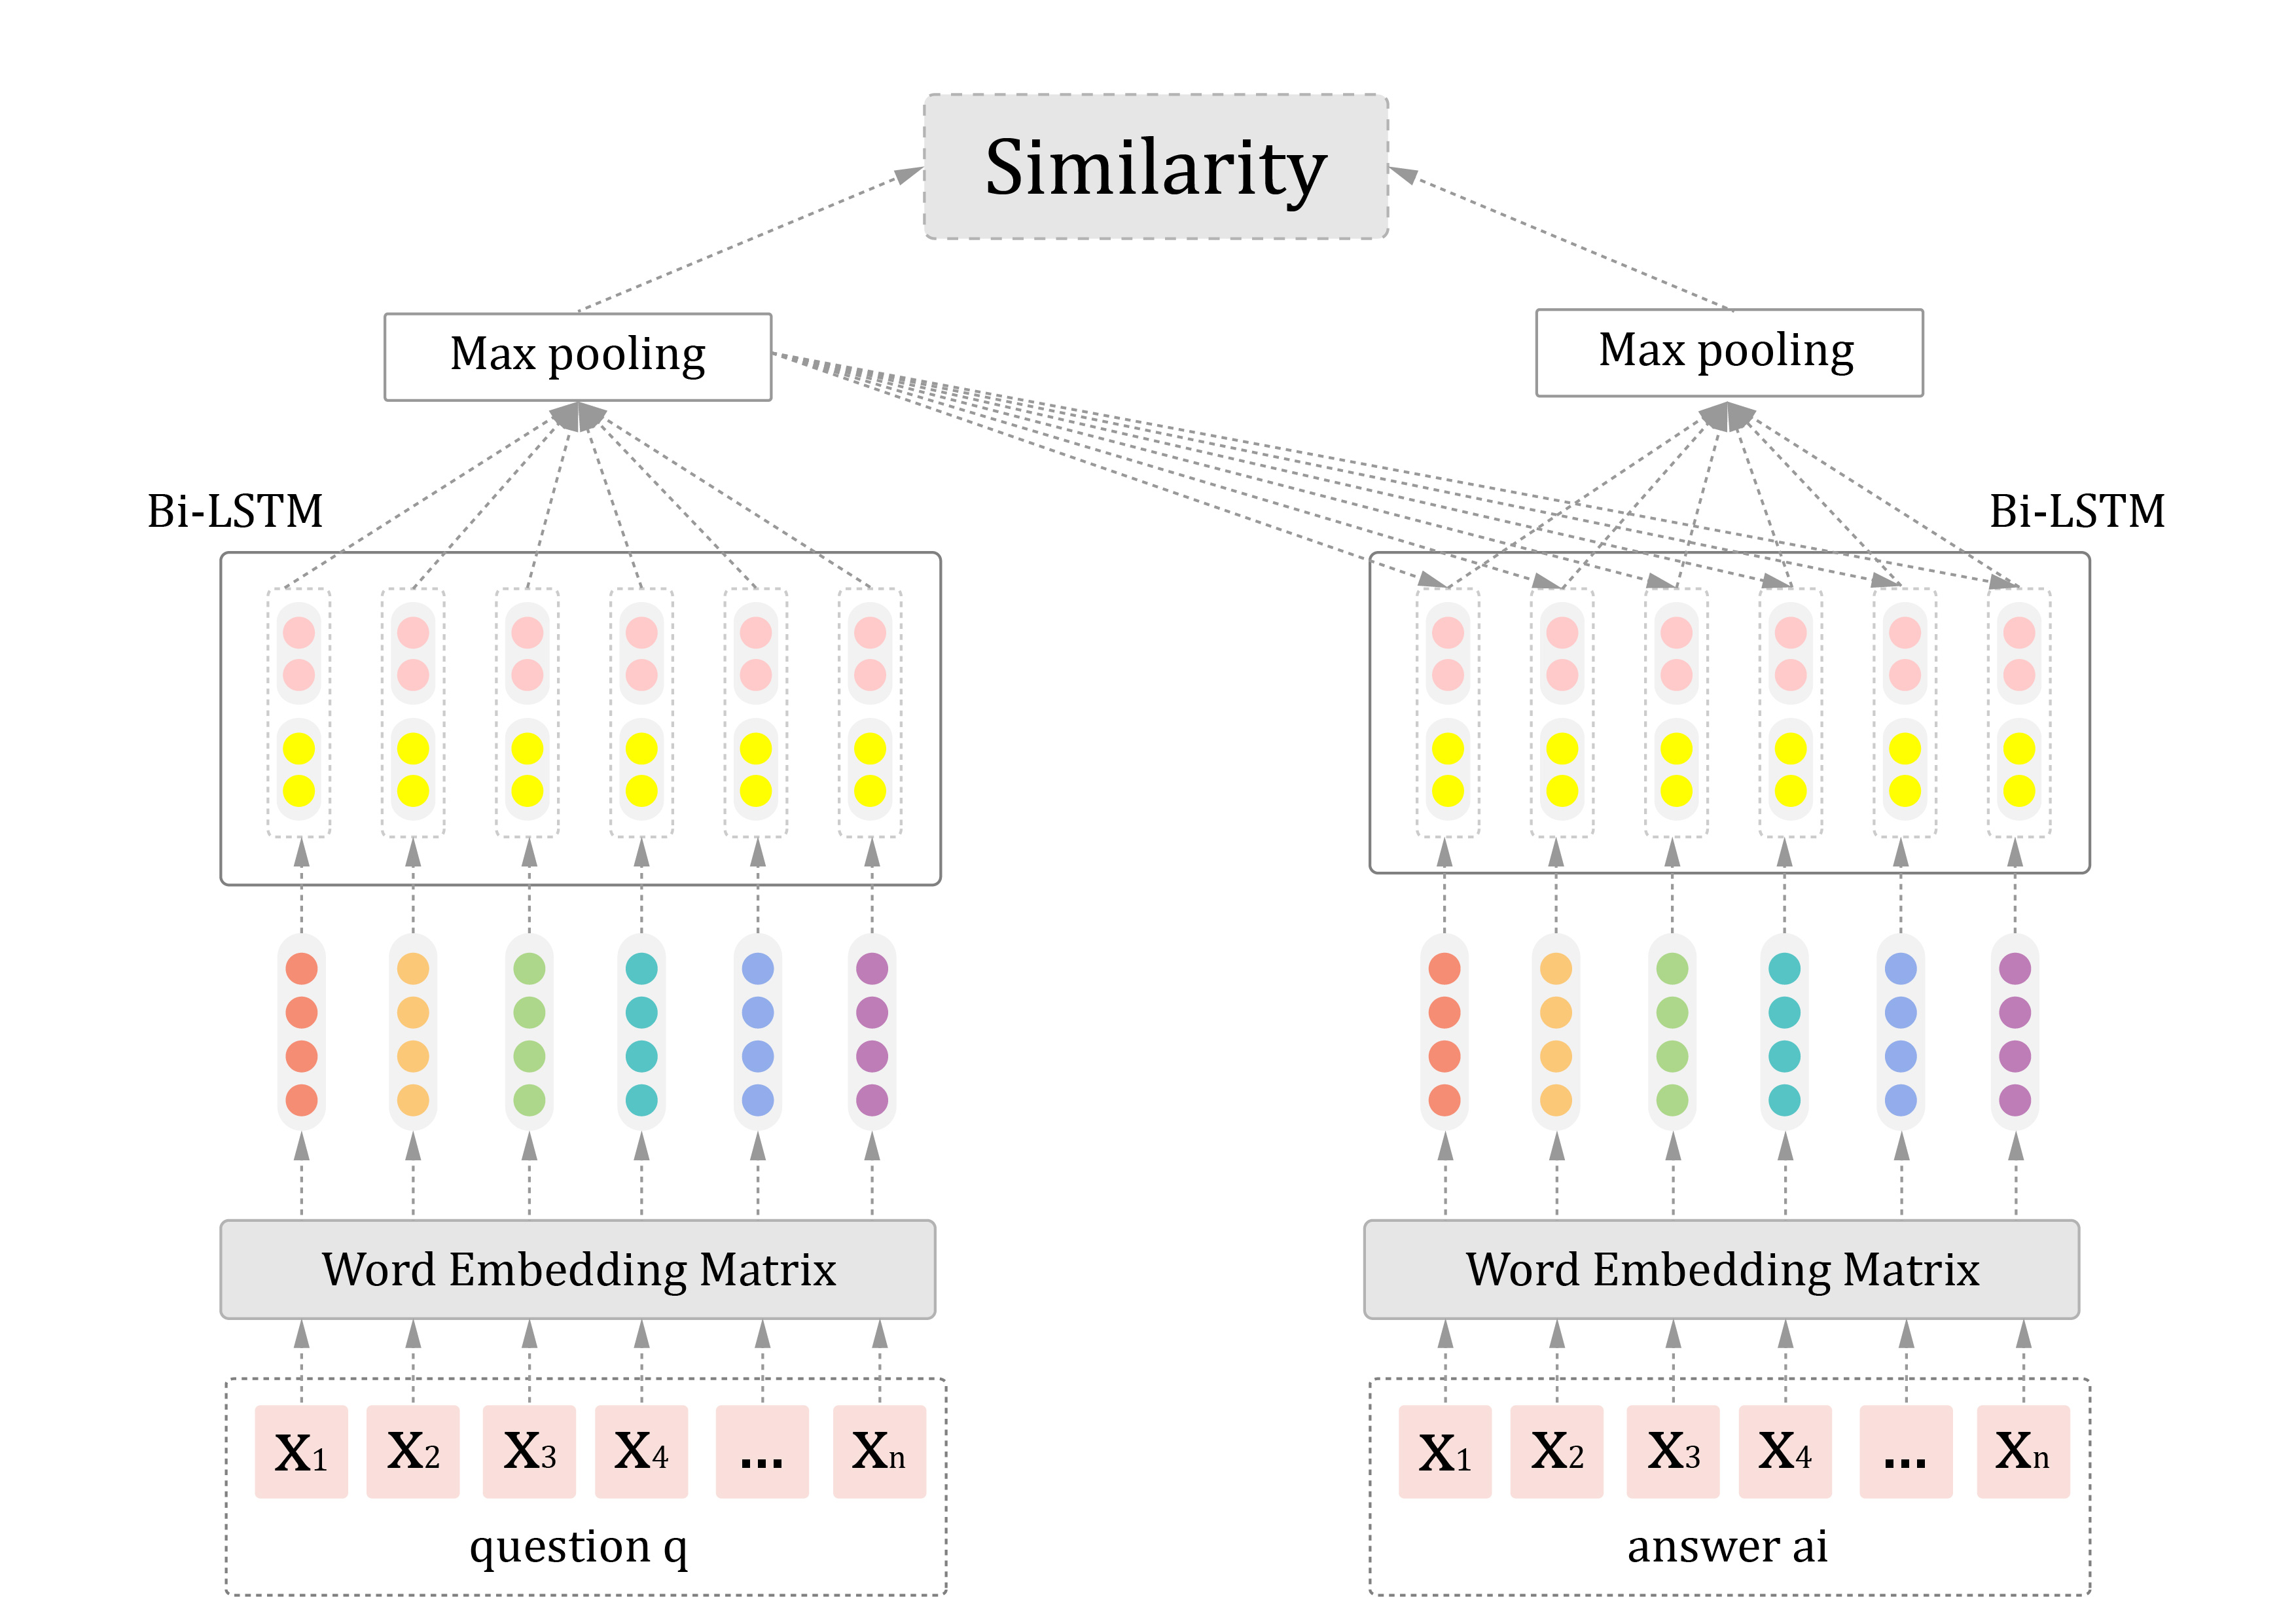
\includegraphics[height=8cm]{resource/qa_bi_lstm}
	\caption{基于Bi-LSTM的问题、答案表示模型}
	\label{fig:qa_bi_lstm}
\end{figure}

 首先生成问题、答案词序列的初始词向量, 然后输入到 Bi-LSTM 网络进入训练,得到问题和答案的最终向量表示, 最后词向量做 max pooling 后通过余弦相似性计算问题、答案向量 矩阵的相关性。实验设置问题、答案的 Bi-LSTM 网 络共享参数, Feng[24]等人的研究表明两个网络共享 参数较两个网络拥有各自不同参数性能更优。
 \\
 
 $\P$基于注意力机制的答案表示
 
与上述模型单独对问题和答案进行表示不同,此节使用一种基本的注意力机制模型,答案中每个词的向量生成均依赖问题,通过动态地将答案中更多的有效信息与问题对齐,可以更好的表示答案与问题之间的依赖关系。 此该注意力机制已在许多自
然语言处理任务上取得不错效果,如机器翻译[25]、事实型问答[26]、句子摘要[20]等。

图 4 为本文基于注意力机制的答案表示模型,模型使用词级别的注意力,如图中描述,在答案端Bi-LSTM 网络输出进入 max pooling 层之前,每个输出会乘以一个基于句子的 Attention 值。 时间 t 时刻, 令答案端的 Bi-LSTM 输出向量为 ,问题词向量为$\textbf{o}_q$,答案中每个词向量$\tilde{\textbf{h}}_{a}(t)$更新如下:
$$
\textbf{m}_{a,q}(t) = \tanh(\textbf{W}_{am}\textbf{h}_{a}(t) + \textbf{W}_{qm}\textbf{o}_q)
\eqno(8)
$$
$$
s_{a,q}(t) = softmax(\textbf{w}_{sm}\textbf{m}_{a,q}(t))
%s_{a,q}(t) = softmax(\textbf{w}_{sm} \tanh(\textbf{W}_{am}\textbf{h}^{a}_t + \textbf{W}_{qm}\textbf{o}_q))
\eqno(9)
$$
$$
\tilde{\textbf{h}}_{a}(t) = \textbf{\textbf{h}}_{a}(t) s_{a,q}(t)
\eqno(10)
$$

其中,$\textbf{W}_{am}$、$\textbf{W}_{qm}$为注意力机制参数矩阵,$\textbf{w}_{sm}$为注意力机制参数向量。从直观上看, 运用注意力机制表示答案相当于一定程度上将答案中与问题关键词相似的词增加权重,给无关词减少权重,使更易于区分正确答案和错误答案。

\begin{figure}[!htb]
	\centering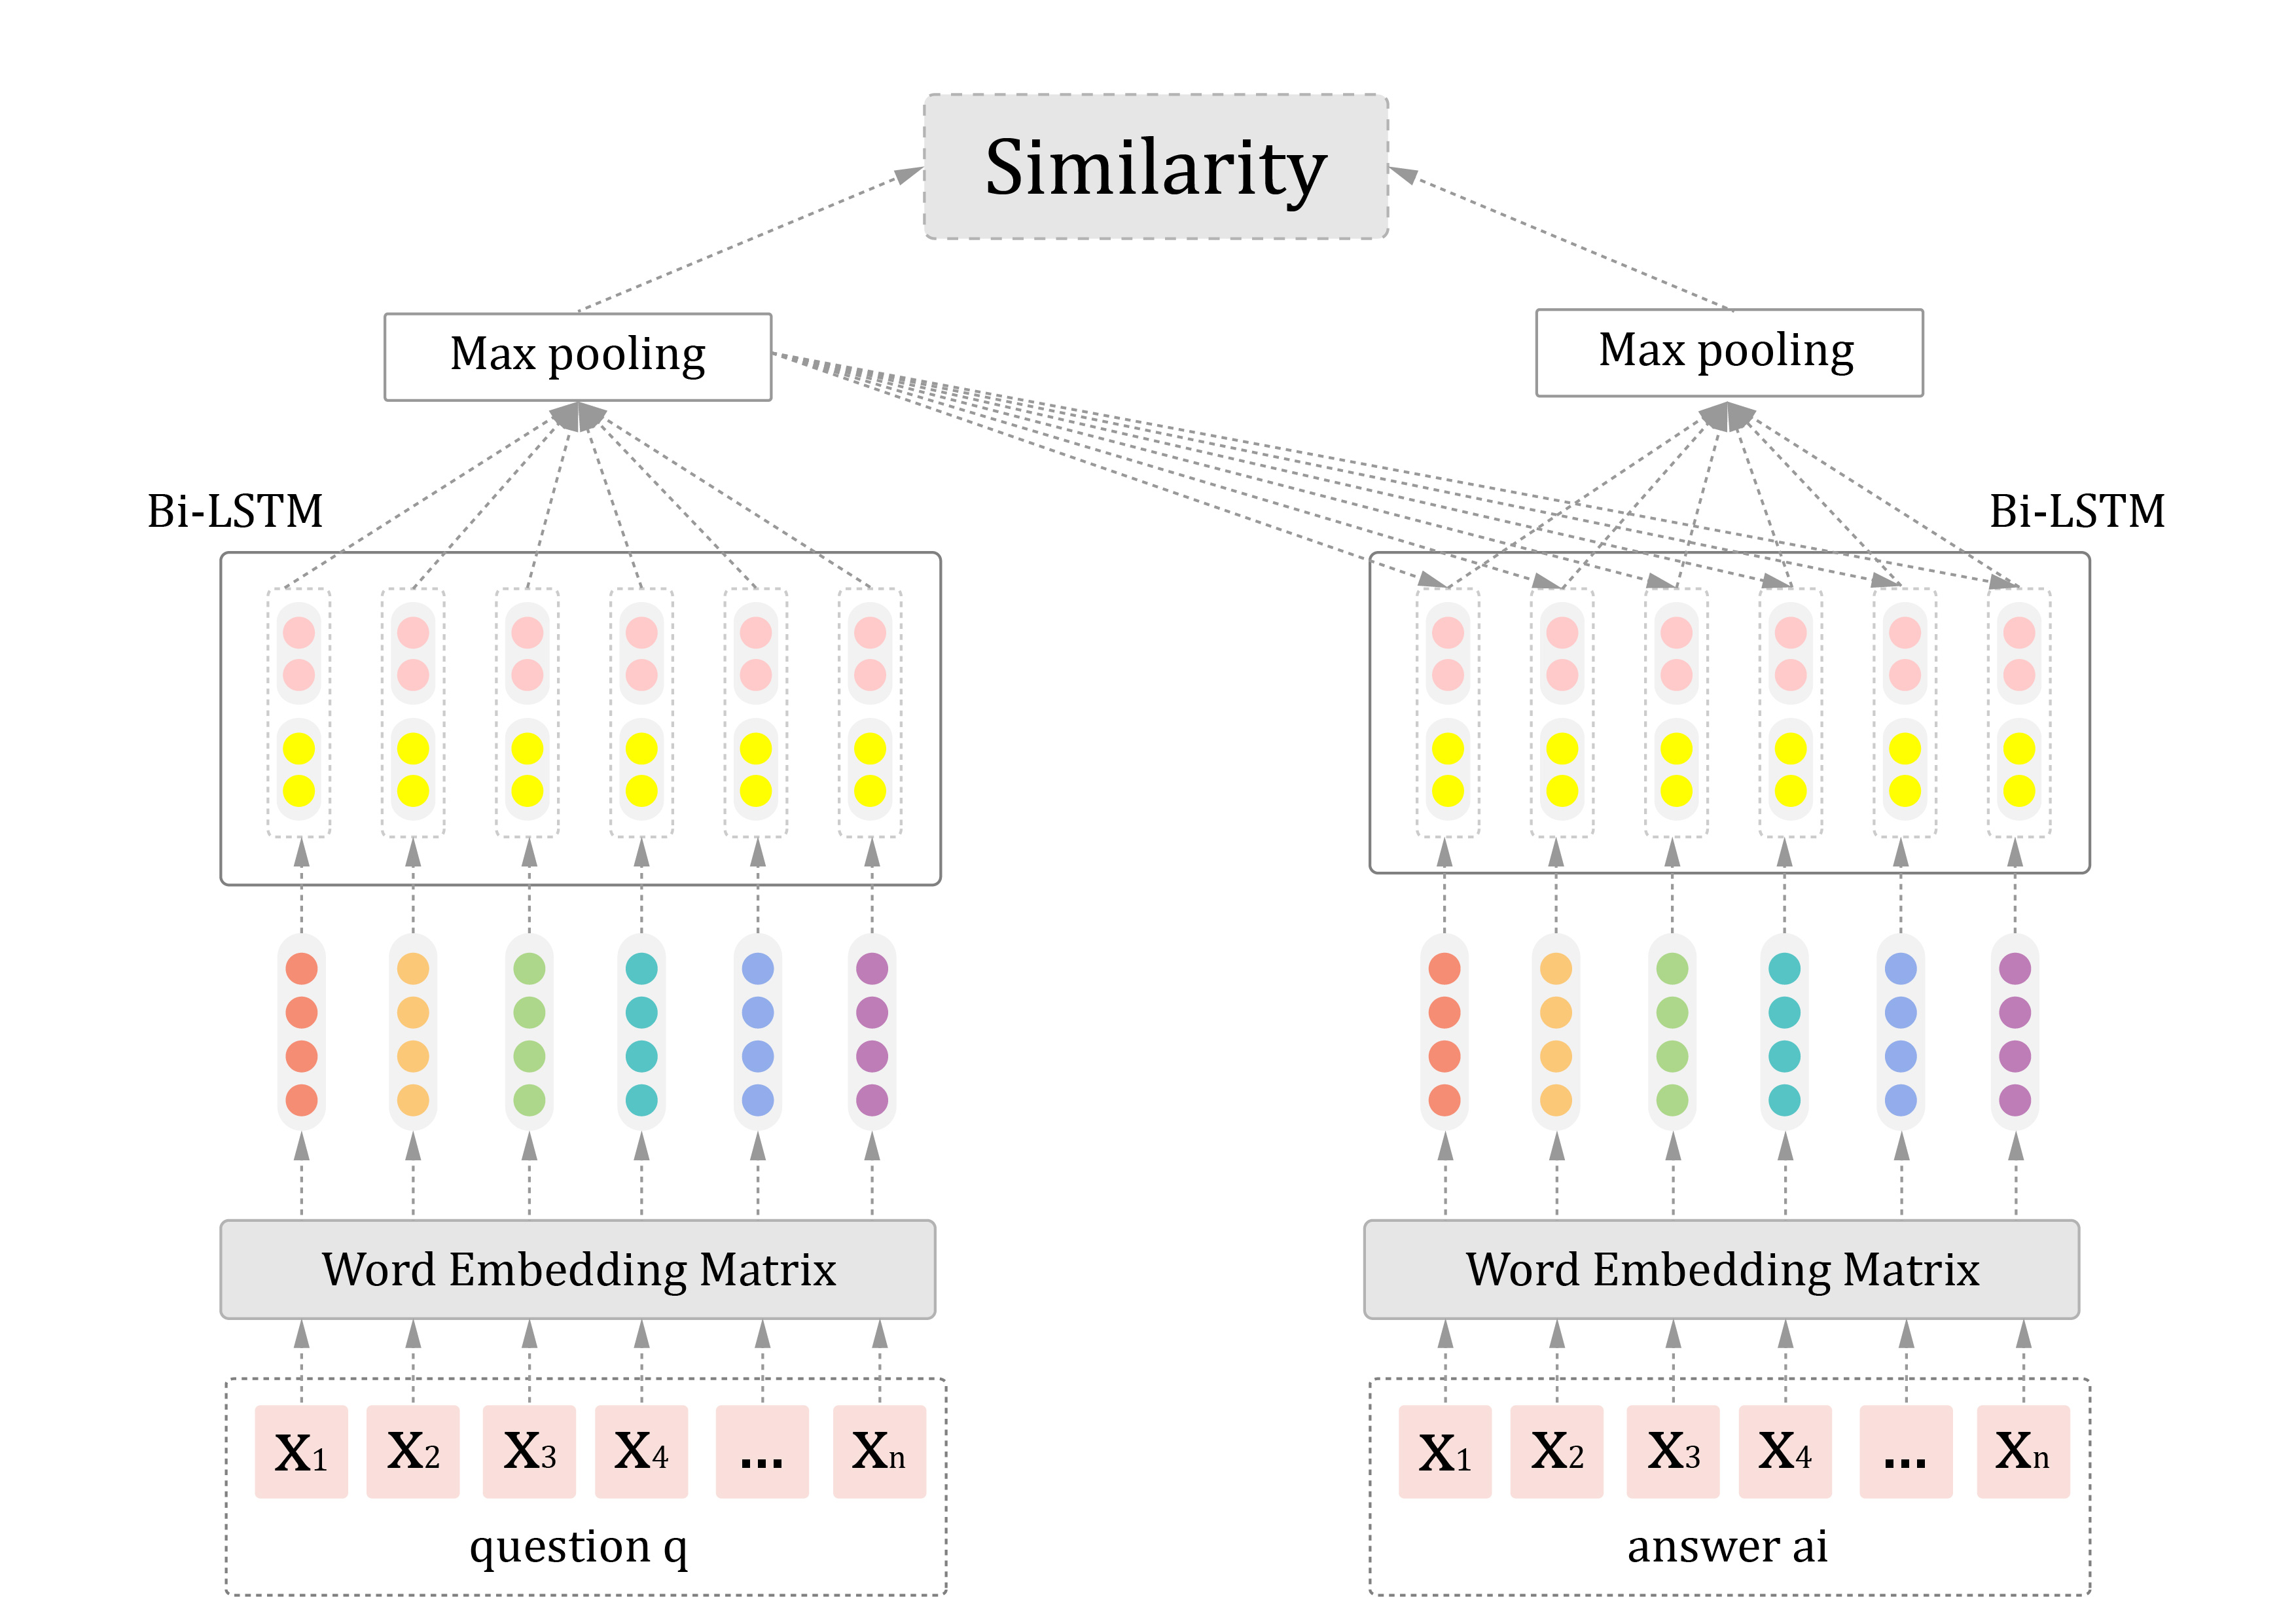
\includegraphics[height=8cm]{resource/qa_attention}
	\caption{基于Attention机制的问题、答案表示模型}
	\label{fig:qa_attention}
\end{figure}


\subsubsection{模型训练}
本文采取问答常见的问答对训练方式(Pairwise Training[27]),训练数据形式为(问题、正确答案、错误答案)。对于某个问题,本文选取一个正确答案作为正例,同时选取k个错误答案作为负例,负例的选择一部分来自主题实体的非答案三元组,另一部分随机从其他问题的正确答案中选取。损失函数使用铰链损失函数(hinge loss),如下:
 $$
\mathcal{L}(q, a_+, a_-) = max \{0, m - S(q, a_+) + S(q, a_-)\}
\eqno(11)
$$

m为正确答案得分和错误得分差距,S(.)为余弦函数,$a_+$为问题的正确答案,$a_-$为问题的错误答案。目标函数为:

$$
\min \sum_q\frac{1}{|P_q|}\sum_{a_+ \in P_q}\sum_{a_- \in N_q} \mathcal{L}(q, a_+, a_-)
\eqno(12)
$$

其中$|P_q|$为问题q的正确答案个数,$N_q$为问题q的k个错误答案集合。本文采取随机梯度下降(stochastic gradient descent,SGD)学习算法。


\subsubsection{最终答案选取策略}
在测试阶段,问答模型给所有候选答案打分排序,然后选择出得分最高答案三元组$S_{max}$,考虑到一个问题的正确答案可能不止一种,因此,本文设置答案阈值,此阈值取损失函数中的m,将得分与最高分相差不超过m的三元组也视作最终答案。如下:$\widehat{A_q}$为最终答案集合,$\hat{a}$为候选答案。
$$
S_{max} = \arg\max_{a \in C_q}{S(q,a)}
\eqno(13)
$$
$$
\widehat{A_q} = \{\hat{a}|S_{max} - S(q, \hat{a}) < m\}
\eqno(14)
$$

\subsection{地理问答实验}
为了评估实验模型,本文使用863项目组构建的基础知识库,同时为了解决目前中文地理领域问题缺乏的问题,本文又构建了较大规模的地理问题测试集,详细在本章数据集小结讲述。先介绍实验相关设置,然后介绍实验结果以及实验分析,最后介绍地理数据集的生成过程。
\subsubsection{参数设置}
实验词向量由word2vec[28]结合最新的中文维基百科语料训练得到,词向量维度为300。实验采取随机梯度下降优化策略,实验尝试过不同的m值,如0.1、0.2、0.3,最终选择0.1。学习率初始值为0.4,每10个epochs下降50$\%$,总共下降4次。剪枝参数max\_grad\_norm设为5,dropout取1.0。实验batch\_size取50,问题负例个数k取20,问题和答案的最大长度设置为50,超出最大长度内容舍弃,双向LSTM隐藏单元设为200。
\subsection{结论}









在给定指称项$m$和指称项对应的候选实体集$E_m=\{e_1,e_2,...,e_n\}$后,计算模型的输入特征:

\begin{enumerate}
	\renewcommand{\labelenumi}{(\theenumi)}
	\item {候选实体$e_i$在知识库中的先验概率,$PriorInKB(m,e_i)$,该特征的定义如公式\ref{eq:popinkb}所示。
		
		\begin{equation}\label{eq:popinkb}
		PriorInKB(m,e_i)=\frac{count(e_i)}{\sum_{e_i\in E_m} {count(e_k)}}
		\end{equation}
		
		其中,$count(e)$表示实体$e$在知识库中作为锚文本出现的次数。
	}
	\item {指称项上下文与候选实体对应词条摘要的文 本相似度,$ContextSimilarity(m,e_i)$,该特征的定义如公式\ref{eq:contex_similarity}所示。
		
		\begin{equation}\label{eq:contex_similarity}
		ContextSimilarity(m,e_i)=\frac{coocurence(m,e_i)}{length(m)}
		\end{equation}
		
		其中,$coocurence(m,e_i)$表示指称项$m$上下文和候选实体$e_i$对应知识库中摘要文本相同的单词数,$length(m)$表示指称项$m$的上下文长度。
	}
	\item {带标注样本集中,候选实体$e_i$的流行度,$PopInCorpus(e_i)$,该特征会随着人工标注的进行而产生变化。该特征的定义如公式\ref{eq:pop_in_corpus}所示。
		
		\begin{equation}\label{eq:pop_in_corpus}
		PopInCorpus(e_i)=\frac{\sum_{anno \in Corpus} {I(anno.e,e_i)}}{sizeof(Corpus)}
		\end{equation}
		
		其中,$anno$表示已标注语料中的一条标注记录,$anno.e$表示标注记录的目标实体。$I(e_i,e_j)$是示值函数,实体$e_i$和实体$e_j$相同则为1,否则为0。$sizeof(Corpus)$表示已标注指称项个数。
	}
	\item{带标注样本集中,候选实体$e_i$作为指称项$m$的目标实体的先验概率,$Prior(m,e_i)$,同上,该特征也会随着标注的进行而产生变化。该特征的定义如公式\ref{eq:prior}所示。
		
		\begin{equation}\label{eq:prior}
		Prior(m,e_i)=\frac{\sum_{anno \in Corpus} {I(anno.e,e_i)\times I(anno.m,m)}}{\sum_{anno \in Corpus} {I(anno.m,m)}}
		\end{equation}
		
		其中,$anno.e$的定义同上。$anno.m$表示标注记录$anno$的指称项。
	}
	\item 指称项名字和候选实体标题的编辑距离,$EDSimarity(m,e_i)$。该特征的定义如公式\ref{eq:ed_simarity}所示。
	
	\begin{equation}\label{eq:ed_simarity}
	EDSimarity(m,e_i)=
	\left\{
	\begin{array}{rcl}
	1       &      & {|length(m)-length(e_i)|=ED(m,e_i)}\\
	0    &      & {\text{其它}}
	\end{array} \right.
	\end{equation}
	
	编辑距离$ED(\cdot,\cdot)$是指两个字符串进行转换时,需要的字符级最少操作次数。编辑距离相似度能够检测指称项和候选实体之间的别名、缩略名等关系。
\end{enumerate}

\subsection{目标实体预测}
在使用监督学习模型$C$处理实体链接任务时,首先需要训练模型$C$。训练样本由带标注的指称项集合构成,例如,带标注的指称$m$包含$n$个候选实体,指称$m$的目标实体是$e^*$,任意一个候选实体$e_i$和指称项$m$组成一 个样本对$\left\langle m,e_i\right\rangle $,若$e_i$是目标实体$e^*$,样本对标记为正例,否则标记为反例。用所有带标注的样本对训练得到模型$C$。

训练得到模型$C$后,对于未标注指称$m$及其候选实体集$E_m$,根据上一节的计算方法获得所有候选实体和指称项组成的样本对的特征向量,模型$C$根据输入的特征向量,计算每个候选实体是目标实体的概率$P_C(e_i|m)$。该预测概率的计算方式和模型的选择相关,例如选择支持向量机模型,可以用样本点距离分类超平面的距离估计正确分类的概率\cite{李航2012统计学习方法};选择人工神经网络模型,可以对输出层每个节点的权值做$softmax$处理,以此获得每个分类标签的分类预测概率\cite{ravuri2016comparative},在此不再一一例举其它模型的预测概率估计方法。取概率最高的候选实体作为指称项$m$的预测实体,如公式\ref{eq:hat_cancidate}所示。

\begin{equation}\label{eq:hat_cancidate}
\hat{e}=\argmax_{e_i\in E_m} P_C(e_i|m)
\end{equation}

然后将该预测实体被正确划分的概率作为指称$m$被正确链接的概率,如公式\ref{eq:predict_prob}所示。

\begin{equation}\label{eq:predict_prob}
P_C(\hat{e}|m)=\max_{e_i\in E_m}P_C(e_i|m)
\end{equation}

\section{实体链接的主动学习算法}
为了减少人工标注的工作量,本文采用基于池的主动学习方法(Pool-based Active Learning)选择实体链接的待标注指称项。主动学习流程图如图\ref{fig:al_overview}所示。

\begin{figure}[!htb]
	\centering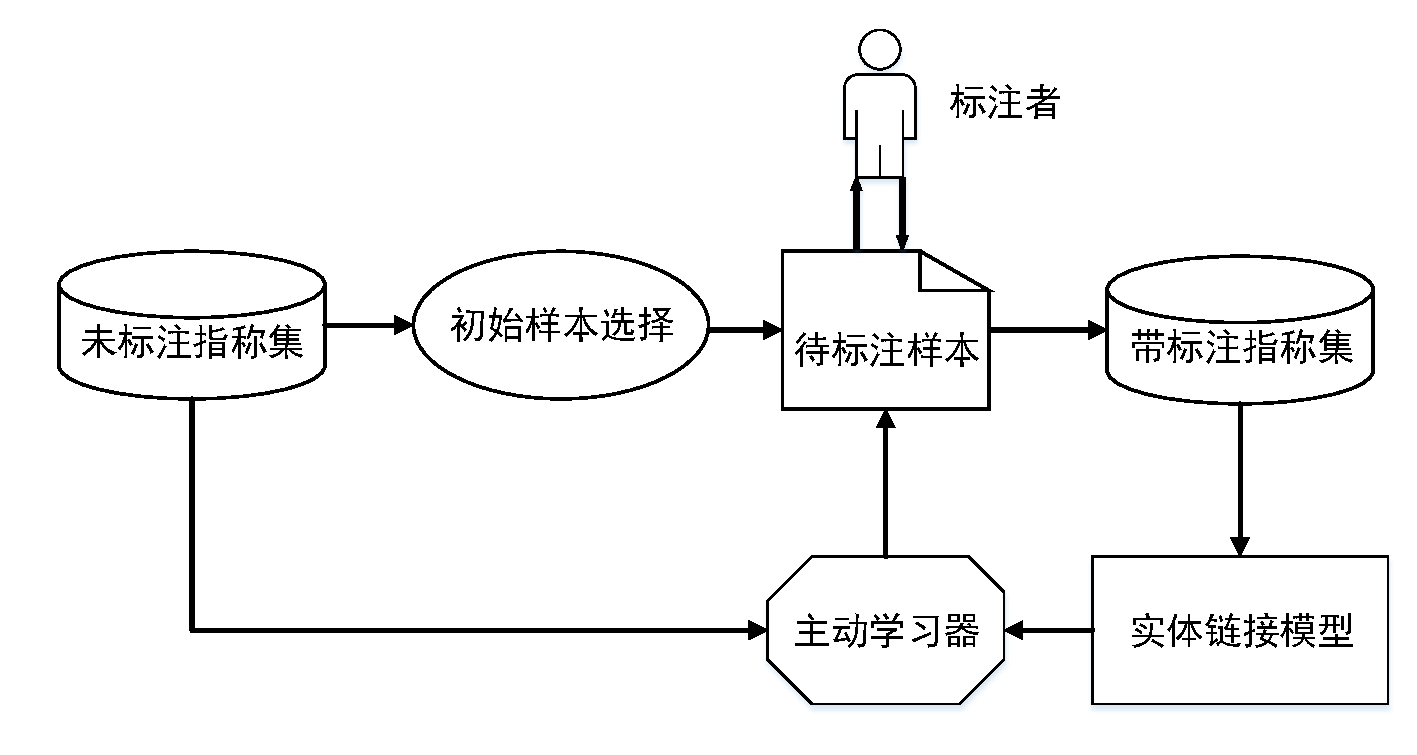
\includegraphics[height=7cm]{resource/al_overview}
	\caption{主动学习流程概览}
	\label{fig:al_overview}
\end{figure}

在每轮迭代训练中,主动学习器能够选出信息量最大的未标注样本集交由人工标注。已有的主动学习\cite{settles2012active}流程如算法\ref{algorithm_AL}所示。在给定未标注训练样本集后, 主动学习进程分为两个阶段,第一阶段的工作是选择初始训练样本集并以此训练初始分类器,第二阶段的工作是选择最佳标注样本并以此迭代训练模型。

\floatname{algorithm}{算法}
\renewcommand{\algorithmicrequire}{\textbf{输入:}} % Use Input in the format of Algorithm
\renewcommand{\algorithmicensure}{\textbf{输出:}} % Use Output in the format of Algorithm
\begin{algorithm}[!htb]
	\caption{基于主动学习的实体链接任务训练进程}
	\label{algorithm_AL}
	\begin{algorithmic}[1] %这个1 表示每一行都显示数字
		\REQUIRE ~ %算法的输入参数:Input
		未标注的指称样本集$ \mathcal{U}=\{m^{(u)} \}_{u=1}^U $
		\ENSURE ~ %算法的输出:Output
		实体链接分类器$C$
		\STATE 从未标注训练集$\mathcal{U}$中选择并标注初始训练样本集$\mathcal{L}_0$\label{al_sup_line1}
		\STATE 利用初始训练样本集$\mathcal{L}_{0}$训练得到弱分类器$C=train(\mathcal{L}_{0})$\label{al_sup_line2}
		\REPEAT \label{al_sup_line3}
		\STATE 从$\mathcal{U}$中找出$k$个信息量最大的样本组成样本集$ \mathcal{U}_{selected} = \{m^{(u)} \}_{u=1}^{k} $\label{al_sup_line4}
		\STATE 对$ \mathcal{U}_{selected}$中的指称进行人工标注得到$ \mathcal{L}_{selected} = \{\left\langle m,e\right\rangle^{(l)} \}_{l=1}^{k} $
		\STATE $ \mathcal{U} = \mathcal{U} \setminus \mathcal{U}_{selected} $
		\STATE $ \mathcal{L}_{t+1} = \mathcal{L}_{t} \cup \mathcal{L}_{selected} $
		\STATE $C=train(\mathcal{L}_{t+1})$
		\UNTIL {达到预期精度或样本集已全部标注} \label{al_sup_line9}
		\RETURN $C$
	\end{algorithmic}
\end{algorithm}

算法第\ref{al_sup_line1}-\ref{al_sup_line2} 行对应主动学习进程的第一个阶段,已有的做法是在未标注样本集$\mathcal{U}$中随机选择待标注样本$\mathcal{U}_{selected}$,然后对这些未标注样本进行人工标注,通过这种方式得到初始带标注样本集$\mathcal{L}_0$,然后用$\mathcal{L}_0$训练得到初始实体链接模型$C$。由于当初始带标注样本集合较小时,通过随机选择的方式获得的子样本集可能无法很好地代表整个样本集。因此,本文对初始训练样本选择方法做了改进,提出基于指称项流行度的初始样本选择方法。

算法第\ref{al_sup_line3}-\ref{al_sup_line9} 行对应主动学习的第二个阶段,其中对于算法第\ref{al_sup_line4}行 信息量度量方法的选择,已有的做法是将样本分类结果的不确定度大小作为信息量的衡量标准,第$t$轮迭代中选出的样本会被加入到带标注样本集$\mathcal{L}_t$中,然后用$\mathcal{L}_t$重新训练模型。在实体链接任务中,仅将不确定度作为选择待标注样本的依据,可能会导致选择过多的离群样本点,不利于模型的训练。因此,本文对迭代训练样本选择方法做了改进,提出综合分类不确定度和指称项流行度的迭代训练样本选择方法。

\section{改进的初始训练样本选择方法}\label{section:al_init_gen}
本节首先对改进的初始训练样本选择方法进行了详细说明,然后给出了该方法对应的算法描述。

\subsection{初始训练样本选择方法}
在主动学习的初始阶段,需要产生一个初始样本集用于训练初始模型。已有的主动学习方法采用随机选择的方式产生初始训练样本集,由于训练样本集相对较小,随机选择的方式很难保证初始样本集的代表性。但是,训练一个性能较好的初始模型对提高主动学习收敛速度非常重要。因此,本文对已有的基于随机选择的初始样本集生成方法做了改进。

为了提高实体链接初始模型的性能,本文提出基于流行度的初始样本选择方法(Sampling by Popularity, SBP)。指称项的流行度按照相同名字的指称项在语料库中出现的频率计算。例如,语料库中包含$n$个指称项,名字为“Jordan”的指称项出现了$m$次,则名字为“Jordan”的所有指称项的流行度为$m/n$。该样本选择方法首先对指称项按照指称项名字分类,计算指称项流行度,然后对指称项流行度高的样本做标注,加入初始训练样本集。该方法的目的是在初始样本选择阶段,尽量选择出现频率较高的指称项,以此保证初始样本集的代表性,从而提高在初始样本集较小的情况下,尽可能提高初始模型的性能。

\subsection{初始训练样本选择算法}
算法\ref{algorithm_init}是对基于流行度的初始样本选择方法的算法描述。初始训练样本的选择分为两个步骤,第一步是不同指称项流行度的统计;第二步是根据指称项流行度选择初始训练样本。

算法第\ref{al_init_line1}-\ref{al_init_line2}行对未标注样本集按指称项名字进行分类,例如所有指称名字为“Jordan”的训练样本都会被划分到集合$\Psi_{Jordan}$中。然后根据集合中的样本数量计算各个指称项在训练集中的流行度,指称项名字相同的样本具有相同的流行度。

算法第\ref{al_init_line3}-\ref{al_init_line7}行对指称项流行度做排序,并在流行度最高的$k$个样本集中分别随机选择一个或多个\footnote{当指称名字数量小于$k$时,需要在一个类簇中选择多个样本,保证最终获得$k$个样本。}样本,经过人工标注后加入初始训练样本集。这样做的目的在于避免初始训练样本集中的样本指称项名字重复度过高,同时保证尽量选择流行度高的指称项样本,从而提高初始训练样本集的代表性。

\floatname{algorithm}{算法}
\renewcommand{\algorithmicrequire}{\textbf{输入:}} % Use Input in the format of Algorithm
\renewcommand{\algorithmicensure}{\textbf{输出:}} % Use Output in the format of Algorithm
\begin{algorithm}[!htb]
	\caption{基于流行度的初始样本集选择算法}
	\label{algorithm_init}
	\begin{algorithmic}[1] %这个1 表示每一行都显示数字
		\REQUIRE ~ %算法的输入参数:Input
		未标注的实体链接样本集$ \mathcal{U}=\{m^{(u)} \}_{u=1}^U $,初始训练集样本个数$k$
		\ENSURE ~ %算法的输出:Output
		初始样本集$\mathcal{L}$
		\STATE 对未标注训练样本按照指称名字$name$分组,指称名字为$name$的样本被分到集合$\Psi_{name}$中\label{al_init_line1}
		\STATE 计算名字为$name$的指称的流行度$\Phi_{name}=\frac{|(\Psi_{name})|}{U}$\label{al_init_line2}
		\STATE 对不同指称的流行度排序,取流行度最高的$k$个指称的名字\label{al_init_line3}
		
		$\mathcal{S}=\{name_1,name_2,...,name_k\}$\label{al_init_line4}
		\FOR {each $name$ in $\mathcal{S}$}
		\STATE 从集合$\Psi_{name}$中随机取一个或多个样本并对其人工标注得到带标注的样本对$L=\left\langle m,e\right\rangle$\label{al_init_line5}
		\STATE $\mathcal{L}=\mathcal{L} \cup \{L\}$
		\ENDFOR\label{al_init_line7}
		\RETURN $\mathcal{L}$
	\end{algorithmic}
\end{algorithm}

\section{改进的迭代训练样本选择方法}\label{section:al_iter_train}
本节首先对改进的迭代训练样本选择方法进行了详细说明,然后给出了该方法对应的算法描述。

\subsection{迭代训练样本选择方法}
在初始训练集上训练得到初始模型后,需要迭代选择信息量最大的未标注样本做标注,然后对模型做重新训练。在已有的主动学习迭代训练样本选择过程中,通常将不确定度最大的样本作为信息量最大的样本,这些样本会交由人工标注并加入下一轮迭代训练,通过这种方式迭代逼近真实模型。本文采用间隔(Margin)度量未标注样本的不确定度。

如公式\ref{eq:margin_confidence}所示 ,$e^{*1}$和$e^{*2}$分别表示在当前模型$C$中,给定指称项$m$,对应置信度最高的和次高的候选实体,以这两个候选实体的置信度差的绝对值作为指称$m$链接到正确实体的置信度。

\begin{align}\label{eq:margin_confidence}
\begin{aligned}
Confidence(m)&=P_C(e^{*1})-P_C(e^{*2})\\
\text{其中,\quad\quad\quad\quad\quad\quad\quad\quad\quad\quad\quad\quad}&\text{\quad\quad\quad\quad\quad\quad\quad\quad\quad\quad\quad\quad\quad\quad\quad\quad}\\
e^{*1}&=\argmax_{E_i\in E_m}P_C(e_i|m)\\
e^{*2}&=\argmax_{E_i\in E_m \setminus \{e^{*1}\}} P_C(e_i|m)
\end{aligned}
\end{align}

易知,$Confidence(m)$越小,表示模型$C$越难正确地从候选实体$e^{*1}$和候选实体$e^{*2}$中区分出目标实体,因此,指称项$m$被正确链接的置信度越小,指称项被正确链接的不确定度越大。指称项链接的不确定度如公式(\ref{eq:margin_uncertainty})所示。

\begin{equation}\label{eq:margin_uncertainty}
Uncertainty(m)=1-Confidence(m)\\
\end{equation}

在本文的实体链接任务中,如果采用仅基于不确定度的样本选择方法来选择待标注样本,则会存在两个缺陷。第一,存在一些不确定度较大,但是在所有样本中处于边缘位置的样本,这些离群样本点不具有代表性,相反还可能会对模型的训练产生负作用,在样本选择过程中,应该尽量避免这类样本点;第二,本文实体链接模型的输入特征向量包含已标注语料中候选实体流行度($PopInCopus(e_i)$)和已标注语料中候选实体先验概率($Prior(e_i|m)$)这两个特征维度,这两个特征都是在已标注样本集上通过统计得到的,因此,带标注的样本分布越离散,带标注样本集中包含的指称项和实体越多,那么上述两个特征维度的统计量越具有代表性。从这个角度看基于不确定度的样本选择算法对这两个特征的计算可能会产生负面影响。因此主动学习的样本选择策略需要在不确定度和多样性之间取一个权衡。为了解决这个问题,本文提出综合不确定度和流行度的样本选择方法(Sampling by Uncertainty and Popularity, SUP)。

\subsection{综合不确定度和流行度的样本选择算法}
接下来给出综合不确定度和流行度的样本选择方法的算法描述。SUP算法是对不确定度和多样性的折衷,如算法\ref{algorithm_iter}所示。

\begin{algorithm}[htb]
	\caption{综合不确定度和流行度样本集选择算法}
	\label{algorithm_iter}
	\begin{algorithmic}[1] %这个1 表示每一行都显示数字
		\REQUIRE ~ %算法的输入参数:Input
		未标注的实体链接样本集$ \mathcal{U}=\{m^{(u)} \}_{u=1}^U $\\
		\quad \quad 选择标注的样本个数$k$
		\ENSURE ~ %算法的输出:Output
		本轮选择标注的训练样本集$ \mathcal{L} $\\
		\STATE $ \mathcal{L} = \{\} $
		\STATE 用K-means聚类法将未标注训练样本集按照指称的流行度划分为$k$类,$Clusters=\{\Psi_1,\Psi_2,...,\Psi_k\}$\label{al_iter_line2}
		\FOR {each $\Psi_i$ in $Clusters$}
		\STATE $m^{*}=\argmax_{m \in \Psi_i} Uncertainty(m)$\label{al_iter_line4}
		\STATE 对$m^{*}$人工标注,得到$\left\langle m^{*},e\right\rangle$
		\STATE $\mathcal{L}=\mathcal{L} \cup \{\left\langle m,e\right\rangle\}$
		\ENDFOR
		\RETURN $ \mathcal{L} $
	\end{algorithmic}
\end{algorithm}

算法第\ref{al_iter_line2}行将所有未标注样本集中的指称项按照指称项流行度进行聚类,完成聚类后,同一个类簇的样本流行度相近。

算法第\ref{al_iter_line4}行从各个流行度的类簇中分别选出不确定度最大的样本交由人工标注,这里不确定度的计算方式依然是模型预测的最优候选实体和次优候选实体置信度的间隔。该样本选择算法能够保证各个指称项流行度区间的样本都有均等机会被选中标注,同时又能保证在每个类簇中被选中标注的样本都是这个类簇中不确定度最大的样本,在兼顾所选样本集多样性的同时保证了不确定度。

\section{实验结果与分析}
本节介绍主动学习方法在实体链接模型训练中的实验,说明实验环境、实验所用数据集、评价指标以及实验配置,最后给出了实验结果数据,并对实验结果进行了分析。

\subsection{实验环境}\label{section:dev_env}
硬件环境:

\begin{itemize}
	\item CPU: Intel(R) Core(TM) i7-3770 CPU @ 3.40GHz
	\item Memory: 4$\times$8GB DDR3 1333 ECC
\end{itemize}

软件环境:

\begin{itemize}
	\item CentOS Linux release 7.3.1611 (Core)
	\item IntelliJ IDEA 2016.3
	\item Java 1.8
	\item MySQL 5.6
\end{itemize}

开源工具:

\begin{itemize}
	\item LibSVM\footnote{用于实现支持向量机。}
	\item Weka 3.6\footnote{用于配合LibSVM实现支持向量机训练。}
	\item Stanford NLP\footnote{用于实现英文分词及词干抽取。}
\end{itemize}

\subsection{实验数据集}\label{section:dataset}
本文使用的数据集是在\textit{CoNLL'03}的基础上做了实体链接标注的\textit{Aida}数据集。数据集包含 1393 篇文章和28815个可用指称项。本文取20000个指称项作为训练集,其余的指称项作为测试集。

\subsection{评价指标}
本章研究主动学习在实体链接模型训练中的作用,并验证本文提出的基于流行度的初始样本选择方法以及综合不确定度和流行度的迭代训练样本选择方法对减少人工标注样本工作量的效果。实际上数据集中的指称项都已经标注好对应的目标实体,但是在模型训练过程中,本文不直接使用 Aida 数据集的标注结果,只有通过主动学习方法选择的样本的标注结果才会被使用,以此来模拟人工标注的过程。本章实验分为以下两个方面:

(1) 以随机选择方法为基线方法,评价基于流行度的初始样本选择方法在标注相同数量样本的前 下,对初始模型性能提升的效果。

(2) 以随机选择法为基线方法,评价基于不确定度的样本选择方法以及综合不确定度和流行度的样本选择方法对模型训练收敛速度的提升效果。

本文对各种样本选择方法好坏的评价指标为主动学习过程中,由主动学习器选择的训练样本所训练得到的模型在测试集里的性能表现,性能表现体现在测试集上实体链接的正确率,计算方法如公式\ref{eq:sup_al_p}所示。

\begin{equation}\label{eq:sup_al_p}
\text{准确率}(P)=\frac{\text{测试集中被正确链接的指称项个数}}{\text{测试集中所有指称项个数}}\times 100\%
\end{equation}

\subsection{模型选择}
本章使用监督学习模型处理实体链接任务,并将该任务作为分类问题来处理。在常用的机器学习分类器中,SVM模型\cite{li2016linking}是目前分类效果较好的模型,其可以通过核函数(本文使用径向基函数(Radial Base Function, RBF))将非线性可分的输入空间的特征映射到高维线性可分的空间的特征,以此学习非线性可分模型。此外,样本点距离分类超平面的远近可以作为分类置信度的依据,而主动学习过程中,分类置信度恰好是样本选择策略的考虑因素之一。

综上,本文在实验阶段使用 SVM 模型作为监督学习模型的代表,处理实体链接任务并研究主动学习方法在该任务上发挥的作用。

\subsection{初始训练样本选择方法实验}
为了验证基于指称项流行度的初始训练样本选择方法对提高初始模型性能的效果,在实验环节,分别通过基于随机选择方法(Random)和基于流行度选择方法(SBP)得到初始样本集,对比在不同初始训练样本集大小的情况下,由初始样本集训练得到的初始模型的性能。

实验中,初始样本集大小的设置从 2000 开始,依次以 2000 递增,最大的初始样本集包含 18000 个训练样本。从图\ref{fig:al_sup_init_result}可以看出,在初始样本集较小的时候,基于指称项流行度的样本选择方法比随机样本选择方法在初始模型的性能上有显著的提升,在初始样本集大小为 2000 的时候,性能提升了 10.1\%,在初始样本集大小为 4000 的时候,性能提升了 5.3\%。当初始样本集大小继续增加时,性能提升值逐渐减小,甚至在一些情况下提升值为负。总体来看,当初始样本集较大时,两种初始训练样本选择方法性能差别不大。

\begin{figure}[!htb]
	\centering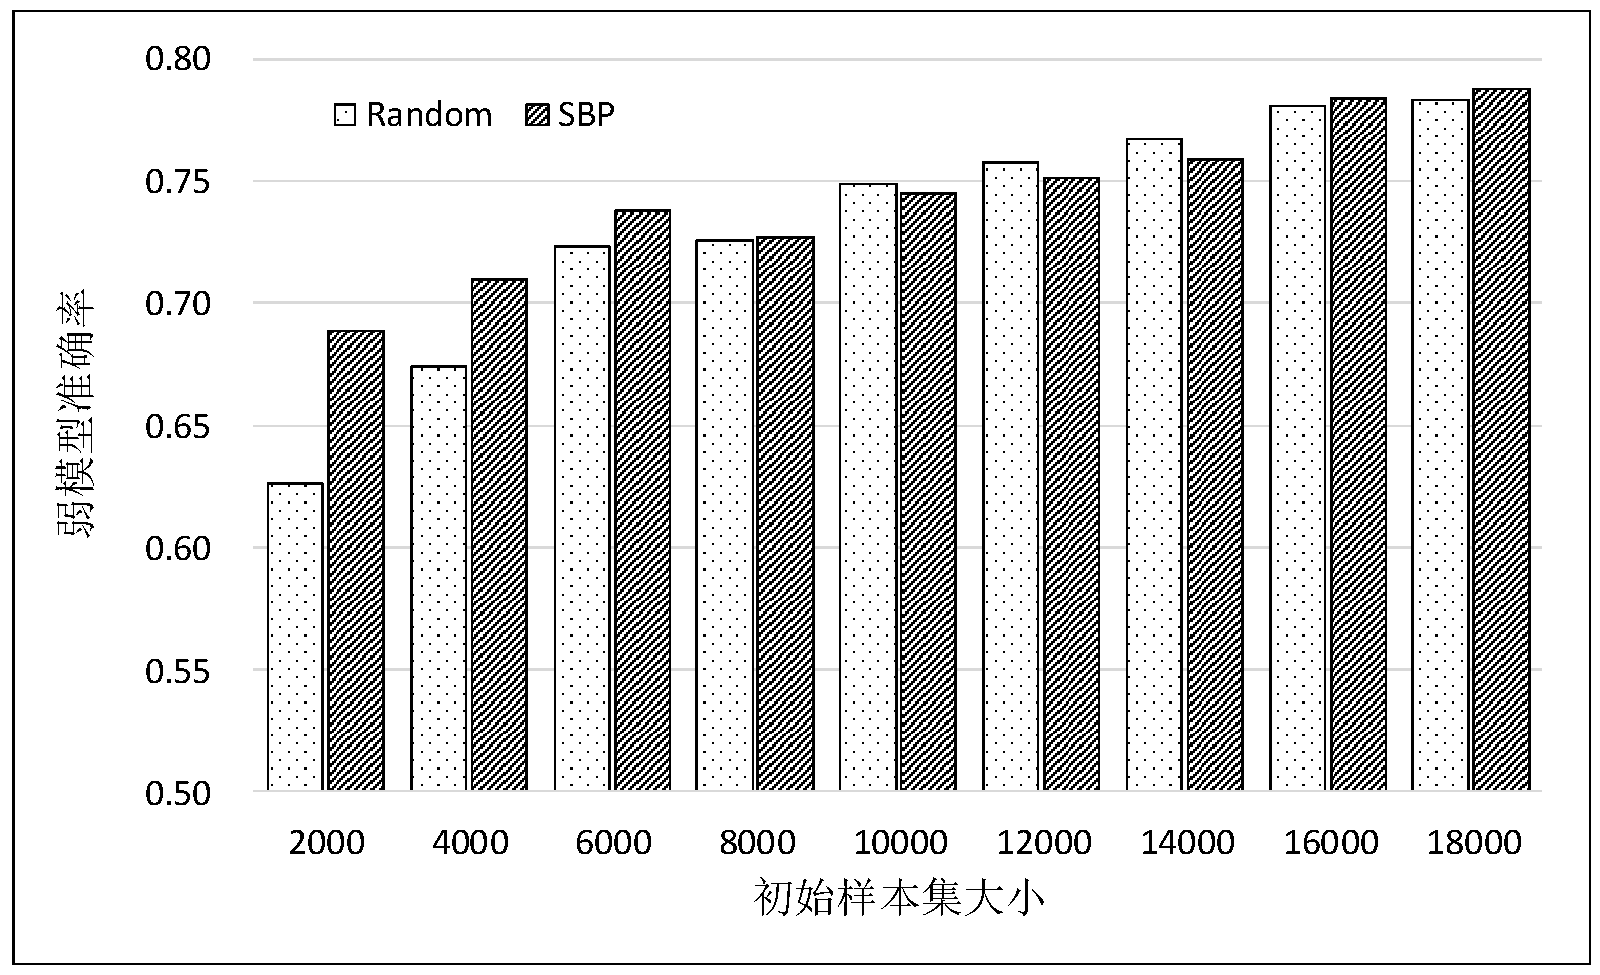
\includegraphics[height=8cm]{resource/surpvised_res1}
	\caption{初始训练样本选择实验结果}
	\label{fig:al_sup_init_result}
\end{figure}

该实验表明,在初始样本集较小的时候,由于样本分布的不均匀特性,随机选择的方法很难选择出能代表整个数据集的样本子集。在实际应用中,用于训练初始模型的初始训练样本集通常较小,使用基于指称项流行度的初始样本选择方法,能有效提升初始模型性能,加快模型在后续训练过程的收敛速度。

\subsection{迭代训练样本选择的实验}
为了验证主动学习方法中不同的样本选择策略对实体链接模型训练的收敛速度的影响,本文在实验环节,对五种不同组合的样本选择策略进行了比较。五种组合如下所示:

(1) Random,初始训练样本和后续迭代训练样本选择都采用随机选择方法,作为基线方法。

(2) Random+Uncertainty,初始训练样本采用随机选择方法,后续迭代训练样本采用基于不确定度的选择方法。

(3) Random+SUP,初始样本采用随机选择方法,后续迭代训练样本采用综合不确定度和流行度的选择方法。

(4) SBP+Uncertainty,初始样本采用基于流行度的选择方法,后续迭代训练样本采用基于不确定度的选择方法。

(5) SBP+SUP,初始样本采用基于流行度的选择方法,后续迭代训练样本采用综合不确定度和流行度的选择方法。

\begin{figure}[!htb]
	\centering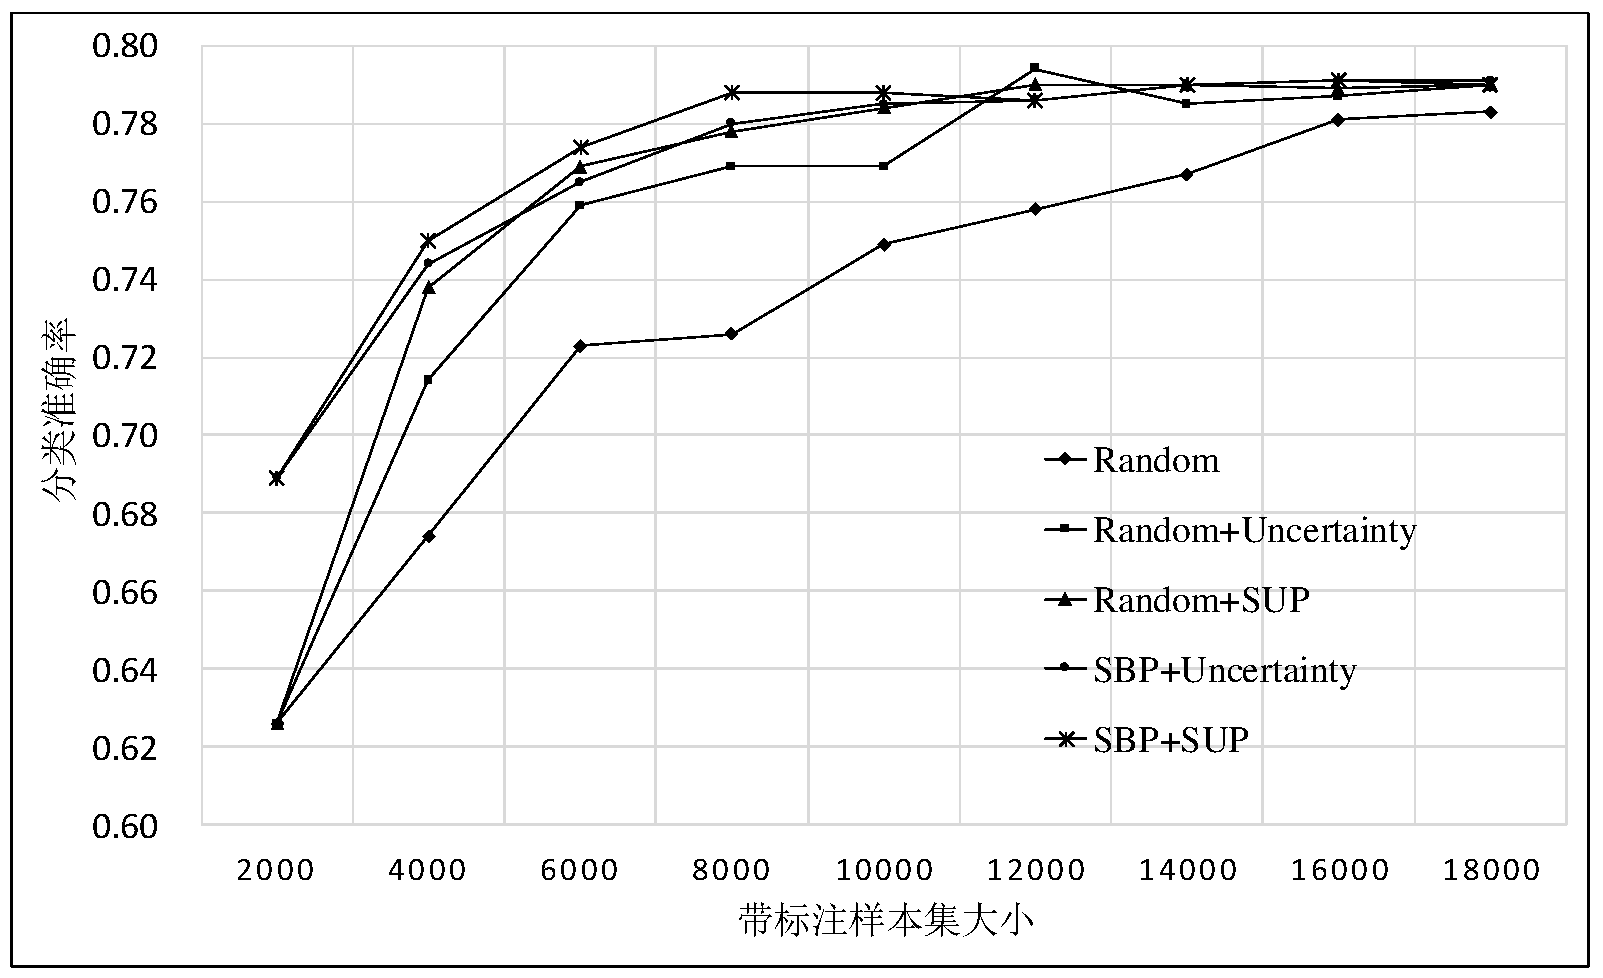
\includegraphics[height=8cm]{resource/surpvised_res2}
	\caption{迭代训练样本选择实验结果}
	\label{fig:al_sup_iter_result}
\end{figure}

从图\ref{fig:al_sup_iter_result}展示的实验结果可以看出,相比随机选择的基线方法,其它四种基于主动学习的样本选择策略对加快模型训练的收敛速度都有显著的提高。证明主动学习方法在实体链接任务中,对减少人工标注样本的工作量确实是有显著效果的。另外,观察曲线走势,综合不确定度和流行度的样本选择方法要优于基于不确定度的样本选择方法,这也验证了基于不确定度的样本选择方法并不能找到最具信息量的样本集,主动学习样本选择过程中需要兼顾不确定度和多样性。

为了量化各种主动学习样本选择策略的表现,采用基于$deficiency$值\cite{schein2007active}的度量方式进行评价,如公式\ref{eq:deficiency}所示。

\begin{equation}\label{eq:deficiency}
Def_n(AL,REF)=\frac{\sum_{t=1}^{n}(acc_n(REF)-acc_t(AL))}{\sum_{t=1}^{n}(acc_n(REF)-acc_t(REF))} \\
\end{equation}

其中,$acc_n(REF)$和$acc_n(AL)$分别表示第$t$轮迭代训练基线方法和主动学习方法训练的模型在测试集上的准确率。主动学习器性能越好,等式分母中$acc_t (AL)$值越大,则等式计算值越小。因此,$Def_n(AL,REF)$越小,主动学习效果越好。

\begin{table}[!htb]
	\caption{主动学习策略结果评价\label{tab:supervised_result2}}
	\centering
	\begin{tabular}{|c|c|c|c|c|}
		\hline
		Random & Random+Uncertainty & Random+SUP & SBP+Uncertainty & SBP+SUP\\
		\hline
		1.000 & 0.552 & 0.369 & 0.274 & \textbf{0.190}\\ 
		\hline
	\end{tabular}
\end{table}

表\ref{tab:supervised_result2}是对主动学习效果的定量分析,无论基于随机的初始样本选择还是基于流行度的初始样本选择,在后续迭代训练中采用基于不确定度和流行度的样本选择算法都能比基于不确定度的样本选择算法得到更快的训练收敛速度。并且采用基于流行度的初始训练样本选择配合综合不确定度和流行度的迭代训练样本选择的策略,$deficiency$值是最低的,性能表现最优。

\section{本章小结}
本章针对实体链接问题,基于主动学习方法,研究了减小人工标注工作量的方法。并且在已有主动学习方法的基础上,针对实体链接任务提出了基于流行度的初始样本选择算法、综合不确定度和流行度的迭代训练样本选择算法。实验结果表明,主动学习方法可以有效地降低实体链接训练集的标注数据,并保持较高的泛化能力。在初始样本集生成阶段,本文提出的选择算法相比随机选择的基线算法初始分类器性能 升了 10.1\%。在主动学习迭代训练阶段,本文 提出的选择算法相比基于不确定度的选择算法$deficiency$值降低了 16.1\%。